\documentclass[../Main.tex]{subfiles}
\begin{document}

% The next for lines makes sure numbering in the appendix is correct - DO NOT CHANGE
\renewcommand{\thesubsection}{\arabic{subsection}}
\renewcommand{\thetable}{\arabic{subsection}.\arabic{table}}
\counterwithin{table}{subsection}
\counterwithin{figure}{subsection}
%--------------------------------------------------------------

\subsection{Summary Statistics}

% Table created by stargazer v.5.2.2 by Marek Hlavac, Harvard University. E-mail: hlavac at fas.harvard.edu
% Date and time: Wed, Mar 27, 2019 - 04:41:55 PM
\begin{table}[!htbp] \centering 
  \caption{Summary statistics for financial variables} 
  \label{compdata} 
\begin{tabular}{@{\extracolsep{5pt}}lccc} 
\\[-1.8ex]\hline 
\hline \\[-1.8ex] 
Statistic & \multicolumn{1}{c}{N} & \multicolumn{1}{c}{Mean} & \multicolumn{1}{c}{St. Dev.} \\ 
\hline \\[-1.8ex] 
Net income (Millions USD) & 20,736 & 392.4 & 1,690.8 \\ 
Revenue (Millions USD) & 17,855 & 4,991.9 & 11,374.3 \\ 
Operation Expenses (Millions USD) & 20,663 & 3,848.5 & 9,512.7 \\ 
Non-Operating Income (Net NO Expenses) (Millions USD) & 20,497 & $-$47.7 & 620.9 \\ 
Google Trends Index (Company Name) & 19,596 & 24.8 & 27.7 \\ 
Google Trends Index (Company Ticker) & 20,359 & 31.1 & 28.5 \\ 
\hline \\[-1.8ex] 
\end{tabular} 
\end{table} 

\begin{table}[!htbp] \centering 
  \caption{Summary of types of data loss} 
  \label{typesofdataloss} 
\begin{tabular}{@{\extracolsep{5pt}}lc} 
\\[-1.8ex]\hline 
\hline \\[-1.8ex] 
Statistic & \multicolumn{1}{c}{Mean} \\ 
\hline \\[-1.8ex] 
Customer & 320 \\ 
Credit Card & 148 \\ 
Social Security Number & 353 \\ 
Name & 423 \\ 
Address & 268 \\ 
Total Breaches & 759 \\ 
\hline \\[-1.8ex] 
\end{tabular} 
\end{table} 

% Table created by stargazer v.5.2.2 by Marek Hlavac, Harvard University. E-mail: hlavac at fas.harvard.edu
% Date and time: Wed, Mar 27, 2019 - 04:41:55 PM
\begin{table}[!htbp] \centering 
  \caption{Summary of magnitude of data loss} 
  \label{recordsdata} 
\begin{tabular}{@{\extracolsep{5pt}}lccccc} 
\\[-1.8ex]\hline 
\hline \\[-1.8ex] 
Statistic & \multicolumn{1}{c}{N} & \multicolumn{1}{c}{Mean} & \multicolumn{1}{c}{Min} & \multicolumn{1}{c}{Max} & \multicolumn{1}{c}{St. Dev.} \\ 
\hline \\[-1.8ex] 
Records leaked per breach & 20,796 & 1,889,737 & 0 & 167,000,000 & 13,959,847 \\ 
\hline \\[-1.8ex] 
\end{tabular} 
\end{table} 

\begin{figure}
    \centering
    \caption{Histogram of number of records leaked per breach}
    \label{recordsleakedfig}
    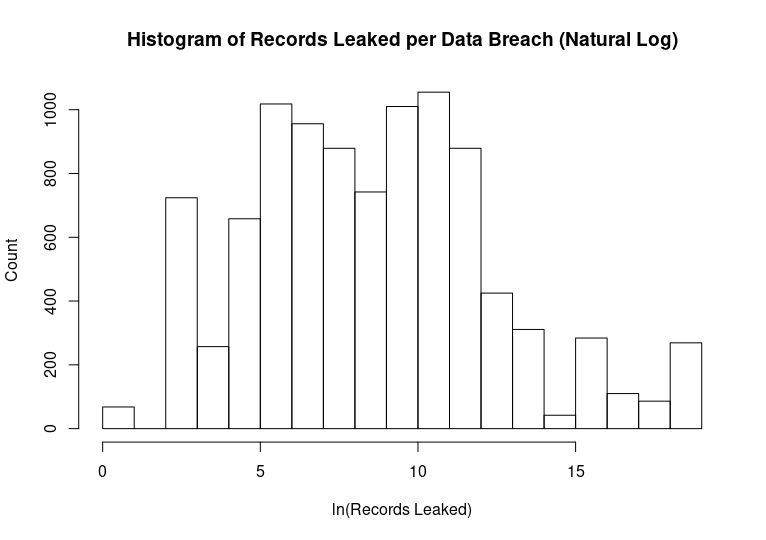
\includegraphics[width=\textwidth]{Images/records_leaked.png}
\end{figure}

\begin{table}[!htbp] \centering 
  \caption{Summary of stock market data} 
  \label{stockdata} 
\begin{tabular}{@{\extracolsep{5pt}}lccc} 
\\[-1.8ex]\hline 
\hline \\[-1.8ex] 
Statistic & \multicolumn{1}{c}{N} & \multicolumn{1}{c}{Mean} & \multicolumn{1}{c}{St. Dev.} \\ 
\hline \\[-1.8ex] 
Daily Firm Return & 936,151 & 0.0005 & 0.03 \\ 
Value Weighted Market Return & 936,404 & 0.0003 & 0.01 \\ 
Risk Free Market Return & 936,404 & 0.04 & 1.19 \\ 
SMB factor & 936,404 & 0.004 & 0.57 \\ 
HML factor & 936,404 & 0.001 & 0.65 \\ 
\hline \\[-1.8ex] 
\end{tabular} 
\end{table} 

\FloatBarrier
\clearpage

\subsection{Revenue}

% Table created by stargazer v.5.2.2 by Marek Hlavac, Harvard University. E-mail: hlavac at fas.harvard.edu
% Date and time: Tue, Mar 26, 2019 - 06:06:53 PM
\begin{table}[!htbp] \centering
  \caption{Revenue: main specification and controls} 
  \label{rev1} 
\resizebox{\textwidth}{!}{\begin{tabular}{@{\extracolsep{5pt}}lccccc} 
\\[-1.8ex]\hline 
\hline \\[-1.8ex] 
 & \multicolumn{5}{c}{\textit{Dependent variable:}} \\ 
\cline{2-6} 
\\[-1.8ex] & \multicolumn{5}{c}{Revenue} \\ 
\\[-1.8ex] & (1) & (2) & (3) & (4) & (5)\\ 
\hline \\[-1.8ex] 
 After Breach & 90.126 & $-$1,075.740$^{*}$ & $-$1,590.337$^{**}$ & $-$25.749 & $-$167.876 \\ 
  & (276.882) & (584.361) & (702.747) & (821.692) & (550.014) \\ 
  & & & & & \\ 
 After Breach x Quarter &  & 44.540$^{**}$ & 52.681$^{**}$ & 47.527$^{**}$ & 44.146$^{**}$ \\ 
  &  & (18.645) & (20.761) & (19.217) & (18.957) \\ 
  & & & & & \\ 
 Records Leaked (log) x After Breach &  &  & 42.130$^{*}$ &  &  \\ 
  &  &  & (24.940) &  &  \\ 
  & & & & & \\ 
 Google Search Index &  &  & 15.579 &  &  \\ 
  &  &  & (9.899) &  &  \\ 
  & & & & & \\ 
 Google Search Index x After Breach &  &  & 11.765 &  &  \\ 
  &  &  & (10.769) &  &  \\ 
  & & & & & \\ 
 After x Revenue Quartile 1 &  &  &  & $-$2,045.009$^{**}$ &  \\ 
  &  &  &  & (795.993) &  \\ 
  & & & & & \\ 
 After x Revenue Quartile 2 &  &  &  & $-$1,660.845$^{**}$ &  \\ 
  &  &  &  & (804.454) &  \\ 
  & & & & & \\ 
 After x Revenue Quartile 3 &  &  &  & $-$1,313.745$^{*}$ &  \\ 
  &  &  &  & (773.529) &  \\ 
  & & & & & \\ 
 Customer Data Leaked x After breach &  &  &  &  & $-$1,169.773$^{***}$ \\ 
  &  &  &  &  & (423.595) \\ 
  & & & & & \\ 
 Credit Card Leaked x After breach &  &  &  &  & $-$18.776 \\ 
  &  &  &  &  & (316.451) \\ 
  & & & & & \\ 
 SSN Leaked x After breach &  &  &  &  & $-$852.194$^{*}$ \\ 
  &  &  &  &  & (478.507) \\ 
  & & & & & \\ 
 Name Leaked x After breach &  &  &  &  & $-$344.489 \\ 
  &  &  &  &  & (384.326) \\ 
  & & & & & \\ 
 Address Leaked x After breach &  &  &  &  & 607.888$^{**}$ \\ 
  &  &  &  &  & (293.087) \\ 
  & & & & & \\ 
\hline \\[-1.8ex] 
Dependent Mean & 5149.94 & 5149.94 & 5149.94 & 5149.94 & 5149.94 \\ 
Dependent SD & 11548.84 & 11548.84 & 11548.84 & 11548.84 & 11548.84 \\ 
Observations & 10,574 & 10,574 & 10,023 & 10,574 & 10,574 \\ 
R$^{2}$ & 0.943 & 0.943 & 0.942 & 0.944 & 0.944 \\ 
Adjusted R$^{2}$ & 0.940 & 0.941 & 0.940 & 0.941 & 0.941 \\ 
\hline 
\hline \\[-1.8ex] 
\textit{Note:}  & \multicolumn{5}{r}{$^{*}$p$<$0.1; $^{**}$p$<$0.05; $^{***}$p$<$0.01} \\ 
 & \multicolumn{5}{r}{Standard errors clustered at the company level} \\ 
 & \multicolumn{5}{r}{Company and quarter fixed effects in all specifications} \\ 
 & \multicolumn{5}{r}{Prediction period is up to 10 years before breach, and event period up to 1 year after} \\ 
\end{tabular}}
\end{table} 

% Table created by stargazer v.5.2.2 by Marek Hlavac, Harvard University. E-mail: hlavac at fas.harvard.edu
% Date and time: Tue, Mar 26, 2019 - 06:06:54 PM
\begin{table}[!htbp] \centering 
  \caption{Revenue: various event period lengths (robustness check)} 
  \label{rev2} 
\resizebox{\textwidth}{!}{\begin{tabular}{@{\extracolsep{5pt}}lcccc} 
\\[-1.8ex]\hline 
\hline \\[-1.8ex] 
 & \multicolumn{4}{c}{\textit{Dependent variable:}} \\ 
\cline{2-5} 
\\[-1.8ex] & \multicolumn{4}{c}{Revenue (Event Period)} \\ 
 & (6 Months) & (1 Year) & (2 Years) & (3 Years) \\ 
\hline \\[-1.8ex] 
 After Breach & $-$915.479 & $-$1,075.740$^{*}$ & $-$1,070.575$^{*}$ & $-$1,000.952$^{*}$ \\ 
  & (561.245) & (584.361) & (595.469) & (591.975) \\ 
  & & & & \\ 
 After Breach x Quarter & 44.145$^{**}$ & 44.540$^{**}$ & 38.889$^{**}$ & 34.038$^{*}$ \\ 
  & (18.661) & (18.645) & (18.954) & (18.679) \\ 
  & & & & \\ 
\hline \\[-1.8ex] 
Dependent Mean & 4969.33 & 5149.94 & 5285.29 & 5340.45 \\ 
Dependent SD & 11224.58 & 11548.84 & 11839.15 & 12066.49 \\ 
Observations & 9,623 & 10,574 & 12,114 & 13,369 \\ 
R$^{2}$ & 0.944 & 0.943 & 0.940 & 0.938 \\ 
Adjusted R$^{2}$ & 0.941 & 0.941 & 0.937 & 0.936 \\ 
\hline 
\hline \\[-1.8ex] 
\textit{Note:}  & \multicolumn{4}{r}{$^{*}$p$<$0.1; $^{**}$p$<$0.05; $^{***}$p$<$0.01} \\ 
 & \multicolumn{4}{r}{Standard errors clustered at the company level} \\ 
 & \multicolumn{4}{r}{Company and quarter fixed effects in all specifications} \\ 
\end{tabular}} 
\end{table} 

% Table created by stargazer v.5.2.2 by Marek Hlavac, Harvard University. E-mail: hlavac at fas.harvard.edu
% Date and time: Wed, Mar 27, 2019 - 05:16:09 PM
\begin{table}[!htbp] \centering 
  \caption{Revenue: first data breaches for each firm (robustness check)} 
  \label{rev3} 
\resizebox{\textwidth}{!}{\begin{tabular}{@{\extracolsep{5pt}}lcccc} 
\\[-1.8ex]\hline 
\hline \\[-1.8ex] 
 & \multicolumn{4}{c}{\textit{Dependent variable:}} \\ 
\cline{2-5} 
\\[-1.8ex] & \multicolumn{4}{c}{Revenue (Event Period)} \\ 
 & (6 Months) & (1 Year) & (2 Years) & (3 Years) \\ 
\hline \\[-1.8ex] 
 After Breach & $-$179.939 & $-$220.091 & $-$235.265 & $-$171.523 \\ 
  & (293.063) & (306.158) & (282.210) & (278.508) \\ 
  & & & & \\ 
 After Breach x Quarter & 10.889 & 13.349 & 14.222$^{*}$ & 12.265 \\ 
  & (8.186) & (8.871) & (8.380) & (9.125) \\ 
  & & & & \\ 
\hline \\[-1.8ex] 
Dependent Mean & 3179.51 & 3227.27 & 3280.89 & 3261.11 \\ 
Dependent SD & 7995.85 & 8143.4 & 8456.55 & 8621.45 \\ 
Observations & 7,432 & 8,035 & 9,077 & 9,941 \\ 
R$^{2}$ & 0.955 & 0.954 & 0.955 & 0.952 \\ 
Adjusted R$^{2}$ & 0.953 & 0.952 & 0.952 & 0.949 \\ 
\hline 
\hline \\[-1.8ex] 
\textit{Note:}  & \multicolumn{4}{r}{$^{*}$p$<$0.1; $^{**}$p$<$0.05; $^{***}$p$<$0.01} \\ 
 & \multicolumn{4}{r}{Standard errors clustered at the company level} \\ 
 & \multicolumn{4}{r}{Company and quarter fixed effects in all specifications} \\ 
\end{tabular}} 
\end{table} 

% Table created by stargazer v.5.2.2 by Marek Hlavac, Harvard University. E-mail: hlavac at fas.harvard.edu
% Date and time: Thu, Mar 28, 2019 - 05:34:59 PM
\begin{table}[!htbp] \centering 
  \caption{Revenue: breakdown by number of data breaches a firm has} 
  \label{rev4} 
\resizebox{\textwidth}{!}{\begin{tabular}{@{\extracolsep{5pt}}lcccc} 
\\[-1.8ex]\hline 
\hline \\[-1.8ex] 
 & \multicolumn{4}{c}{\textit{Dependent variable:}} \\ 
\cline{2-5} 
\\[-1.8ex] & \multicolumn{4}{c}{Revenue (Number of Breaches for Firm)} \\ 
 & (1) & (2) & (3) & (4+) \\ 
\hline \\[-1.8ex] 
 After Breach & $-$125.512 & $-$479.309 & $-$321.079 & $-$624.802 \\ 
  & (157.839) & (916.204) & (438.449) & (1,884.327) \\ 
  & & & & \\ 
 After Breach x Quarter & 9.659 & 5.170 & 18.815 & 82.551 \\ 
  & (6.522) & (23.129) & (12.656) & (52.310) \\ 
  & & & & \\ 
\hline \\[-1.8ex] 
Number of Data Breaches  & 231 & 139 & 85 & 176 \\ 
Dependent Mean & 1933.71 & 7302.19 & 5438.41 & 15062.09 \\ 
Dependent SD & 5942.93 & 14370.67 & 5799.58 & 18875.12 \\ 
Observations & 5,826 & 2,348 & 1,050 & 1,350 \\ 
R$^{2}$ & 0.955 & 0.940 & 0.926 & 0.929 \\ 
Adjusted R$^{2}$ & 0.952 & 0.937 & 0.920 & 0.925 \\ 
\hline 
\hline \\[-1.8ex] 
\textit{Note:}  & \multicolumn{4}{r}{$^{*}$p$<$0.1; $^{**}$p$<$0.05; $^{***}$p$<$0.01} \\ 
 & \multicolumn{4}{r}{Standard errors clustered at the company level} \\ 
 & \multicolumn{4}{r}{Company and quarter fixed effects in all specifications} \\ 
 & \multicolumn{4}{r}{Prediction period is up to 10 years before breach, and event period up to 1 year after} \\ 
\end{tabular}} 
\end{table} 

% Table created by stargazer v.5.2.2 by Marek Hlavac, Harvard University. E-mail: hlavac at fas.harvard.edu
% Date and time: Wed, Mar 27, 2019 - 04:10:49 PM
\begin{table}[!htbp] \centering 
  \caption{Revenue: offset event dates (robustness check)} 
  \label{rev5} 
\resizebox{\textwidth}{!}{\begin{tabular}{@{\extracolsep{5pt}}lccccc} 
\\[-1.8ex]\hline 
\hline \\[-1.8ex] 
 & \multicolumn{5}{c}{\textit{Dependent variable:}} \\ 
\cline{2-6} 
\\[-1.8ex] & \multicolumn{5}{c}{Revenue (Offset of Event Date)} \\ 
 & (0) & (-2 Years) & (-3 Years) & (+2 Years) & (+3 Years) \\ 
\hline \\[-1.8ex] 
 After Breach & $-$1,075.740$^{*}$ & $-$729.132$^{*}$ & $-$751.626 & $-$708.919 & $-$1,151.524$^{**}$ \\ 
  & (584.361) & (424.132) & (752.797) & (578.295) & (543.060) \\ 
  & & & & & \\ 
 After Breach x Quarter & 44.540$^{**}$ & 27.944$^{*}$ & 30.224 & 15.326 & 19.878 \\ 
  & (18.645) & (16.653) & (32.716) & (19.200) & (17.307) \\ 
  & & & & & \\ 
\hline \\[-1.8ex] 
Dependent Mean & 5149.94 & 5149.94 & 5149.94 & 5149.94 & 5149.94 \\ 
Dependent SD & 11548.84 & 11548.84 & 11548.84 & 11548.84 & 11548.84 \\ 
Observations & 10,574 & 6,153 & 4,519 & 13,369 & 14,437 \\ 
R$^{2}$ & 0.943 & 0.957 & 0.957 & 0.938 & 0.937 \\ 
Adjusted R$^{2}$ & 0.941 & 0.954 & 0.954 & 0.936 & 0.935 \\ 
\hline 
\hline \\[-1.8ex] 
\textit{Note:}  & \multicolumn{5}{r}{$^{*}$p$<$0.1; $^{**}$p$<$0.05; $^{***}$p$<$0.01} \\ 
 & \multicolumn{5}{r}{Standard errors clustered at the company level} \\ 
 & \multicolumn{5}{r}{Company and quarter fixed effects in all specifications} \\ 
 & \multicolumn{5}{r}{Prediction period is up to 10 years before breach, and event period up to 1 year after} \\ 
\end{tabular}} 
\end{table} 


\FloatBarrier

\begin{figure}
    \centering
    \caption{Mean residual revenue (fixed effects removed)}
    \label{revfig}
    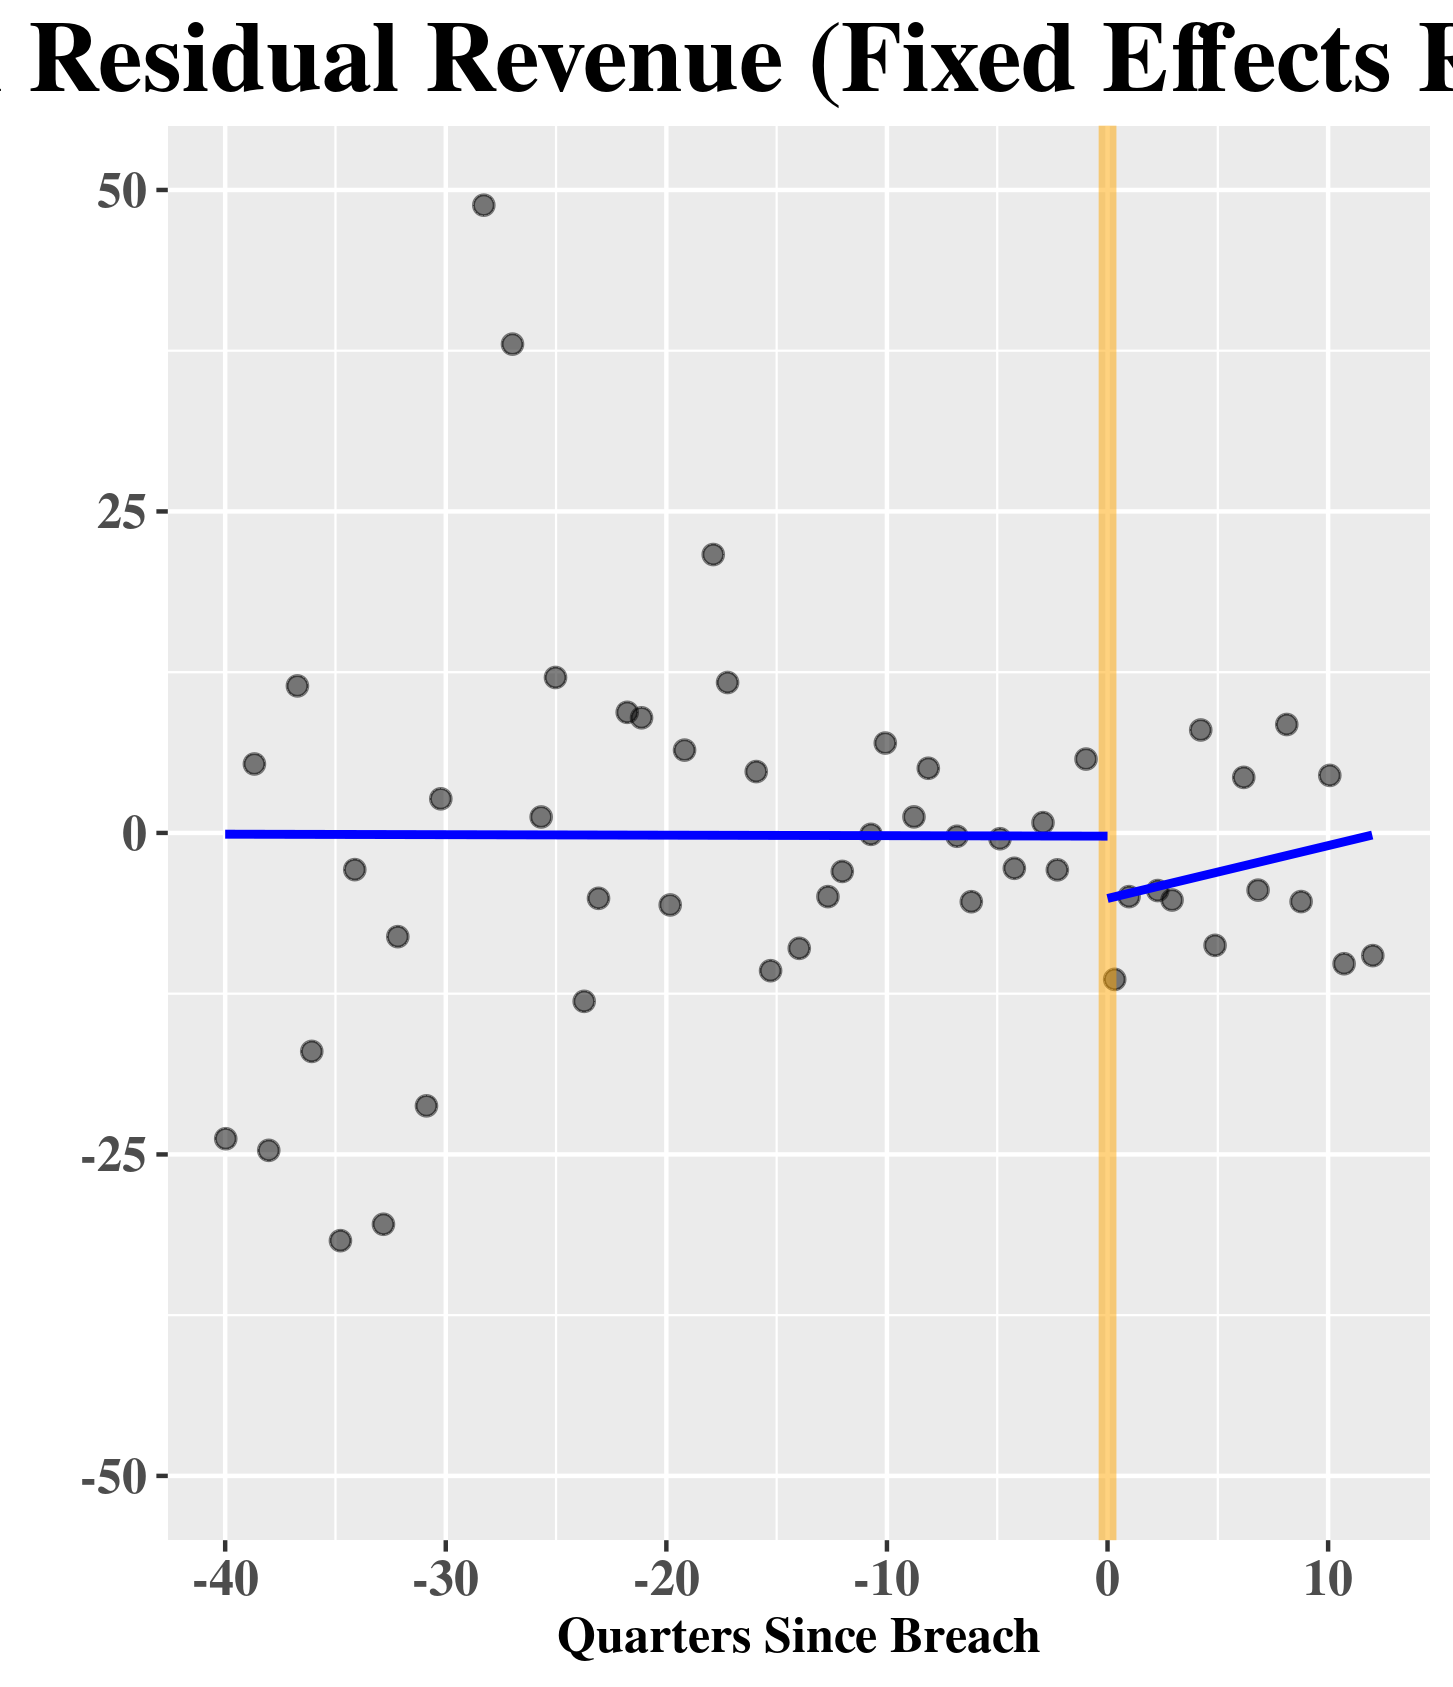
\includegraphics[width=\textwidth]{Images/mean_resid_revenue_3y.png}
\end{figure}

\FloatBarrier
\clearpage

\subsection{Log Revenue}

% Table created by stargazer v.5.2.2 by Marek Hlavac, Harvard University. E-mail: hlavac at fas.harvard.edu
% Date and time: Tue, Mar 26, 2019 - 06:06:55 PM
\begin{table}[!htbp] \centering 
  \caption{Log Revenue: main specification and controls} 
  \label{logrev1} 
\resizebox{\textwidth}{!}{\begin{tabular}{@{\extracolsep{5pt}}lcccc} 
\\[-1.8ex]\hline 
\hline \\[-1.8ex] 
 & \multicolumn{4}{c}{\textit{Dependent variable:}} \\ 
\cline{2-5} 
\\[-1.8ex] & \multicolumn{4}{c}{Log Revenue (Event Period)} \\ 
 & (6 Months) & (1 Year) & (2 Years) & (3 Years) \\ 
\\[-1.8ex] & (1) & (2) & (3) & (4)\\ 
\hline \\[-1.8ex] 
 After Breach & 0.006 & $-$0.006 & $-$0.004 & 0.019 \\ 
  & (0.040) & (0.043) & (0.047) & (0.046) \\ 
  & & & & \\ 
 After Breach x Quarter & 0.001 & 0.001 & 0.001 & 0.00002 \\ 
  & (0.001) & (0.002) & (0.002) & (0.002) \\ 
  & & & & \\ 
\hline \\[-1.8ex] 
Dependent Mean & 6.92 & 6.96 & 6.99 & 6.99 \\ 
Dependent SD & 2.3 & 2.28 & 2.25 & 2.25 \\ 
Observations & 9,623 & 10,574 & 12,114 & 13,369 \\ 
R$^{2}$ & 0.966 & 0.964 & 0.961 & 0.953 \\ 
Adjusted R$^{2}$ & 0.965 & 0.962 & 0.959 & 0.951 \\ 
\hline 
\hline \\[-1.8ex] 
\textit{Note:}  & \multicolumn{4}{r}{$^{*}$p$<$0.1; $^{**}$p$<$0.05; $^{***}$p$<$0.01} \\ 
 & \multicolumn{4}{r}{Standard errors clustered at the company level} \\ 
 & \multicolumn{4}{r}{Company and quarter fixed effects in all specifications} \\ 
\end{tabular}} 
\end{table} 

\FloatBarrier

\begin{figure}
    \centering
    \caption{Mean residual log revenue (fixed effects removed)}
    \label{logrevfig}
    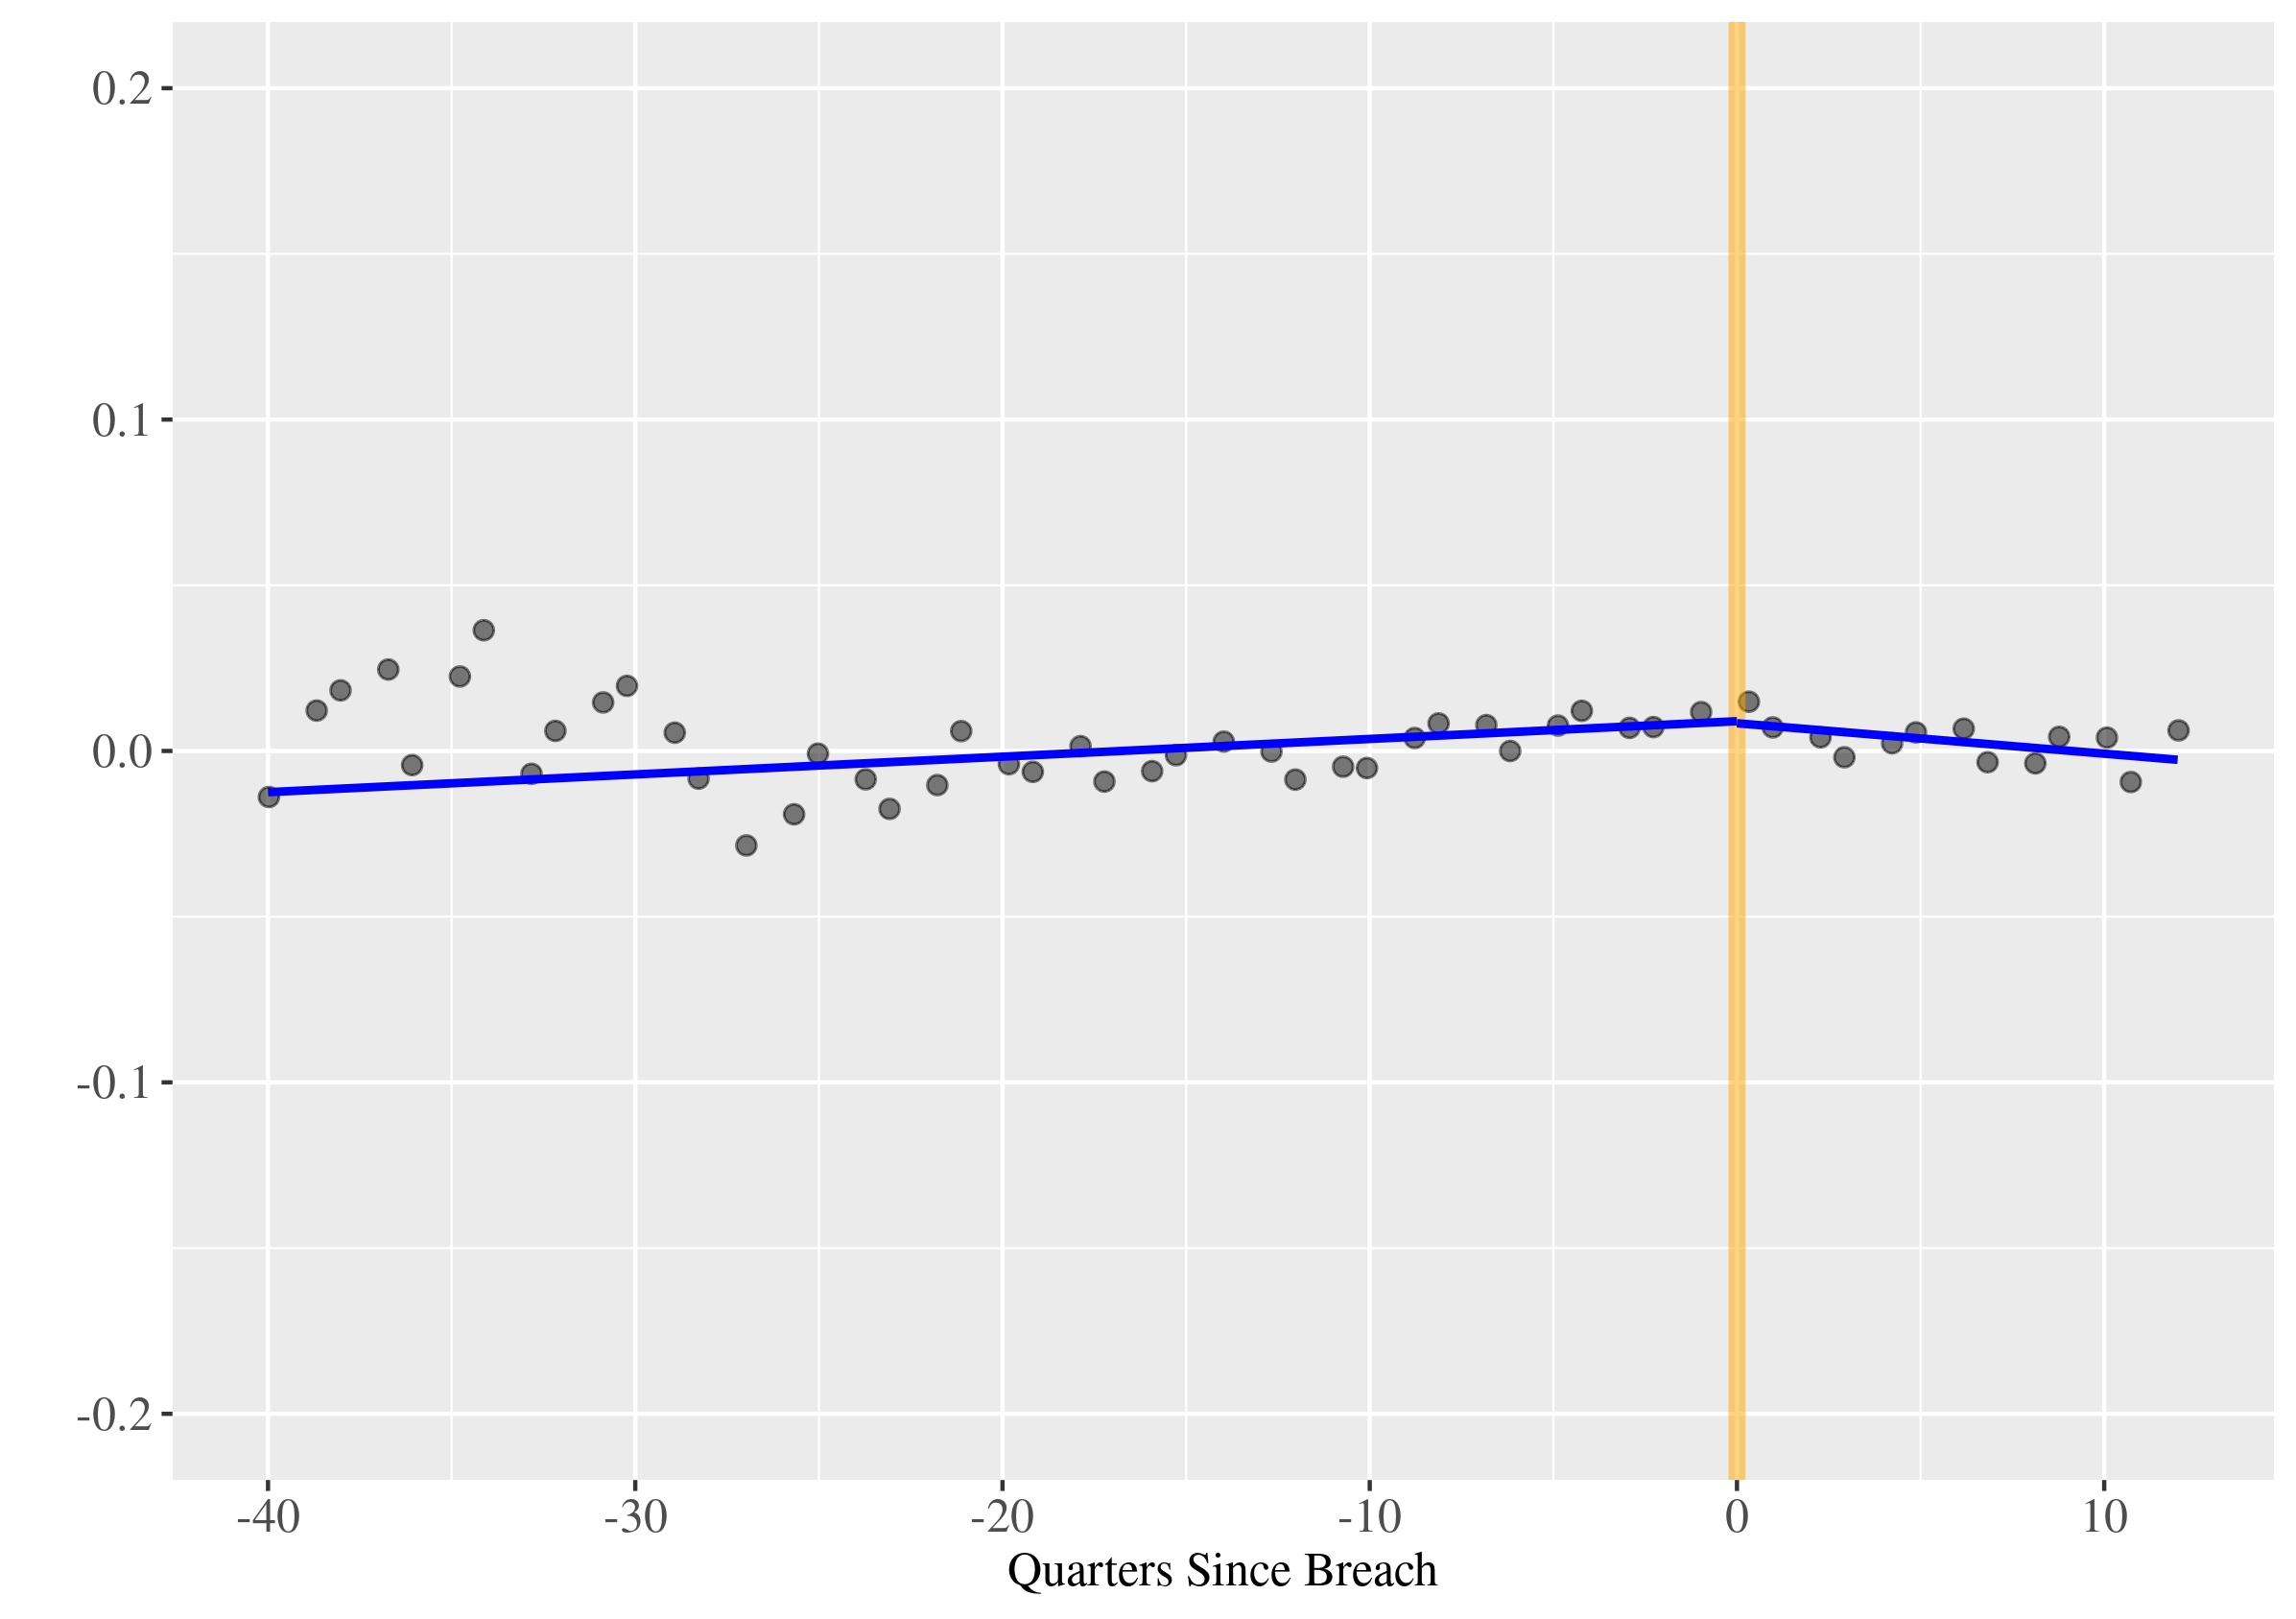
\includegraphics[width=\textwidth]{Images/mean_resid_logrevenue_3y.png}
\end{figure}


\FloatBarrier
\clearpage

\subsection{Non-Operating Income/Expenses}

% Table created by stargazer v.5.2.2 by Marek Hlavac, Harvard University. E-mail: hlavac at fas.harvard.edu
% Date and time: Sun, Mar 31, 2019 - 01:51:16 PM
\begin{table}[!htbp] \centering 
  \caption{Non-operating income: main specification and controls} 
  \label{nop1} 
\resizebox{\textwidth}{!}{\begin{tabular}{@{\extracolsep{5pt}}lccccc} 
\\[-1.8ex]\hline 
\hline \\[-1.8ex] 
 & \multicolumn{5}{c}{\textit{Dependent variable:}} \\ 
\cline{2-6} 
\\[-1.8ex] & \multicolumn{5}{c}{Non-Operating Income --- Net of NO Expenses} \\ 
\\[-1.8ex] & (1) & (2) & (3) & (4) & (5)\\ 
\hline \\[-1.8ex] 
 After Breach & 13.472 & 101.301$^{*}$ & 112.690$^{*}$ & 110.329$^{*}$ & 88.530$^{*}$ \\ 
  & (11.547) & (59.933) & (66.504) & (58.722) & (52.293) \\ 
  & & & & & \\ 
 After Breach x Quarter &  & $-$3.381$^{*}$ & $-$3.708$^{*}$ & $-$3.342$^{*}$ & $-$3.231$^{*}$ \\ 
  &  & (1.930) & (2.157) & (1.947) & (1.844) \\ 
  & & & & & \\ 
 Records Leaked (log) x After Breach &  &  & $-$1.635 &  &  \\ 
  &  &  & (1.402) &  &  \\ 
  & & & & & \\ 
 Google Search Index &  &  & $-$0.834 &  &  \\ 
  &  &  & (0.736) &  &  \\ 
  & & & & & \\ 
 Google Search Index x After Breach &  &  & $-$0.178 &  &  \\ 
  &  &  & (0.313) &  &  \\ 
  & & & & & \\ 
 After x Revenue Quartile 1 &  &  &  & $-$25.918 &  \\ 
  &  &  &  & (28.945) &  \\ 
  & & & & & \\ 
 After x Revenue Quartile 2 &  &  &  & $-$8.147 &  \\ 
  &  &  &  & (20.196) &  \\ 
  & & & & & \\ 
 After x Revenue Quartile 3 &  &  &  & $-$2.787 &  \\ 
  &  &  &  & (20.822) &  \\ 
  & & & & & \\ 
 Customer Data Leaked x After breach &  &  &  &  & $-$50.464$^{*}$ \\ 
  &  &  &  &  & (26.211) \\ 
  & & & & & \\ 
 Credit Card Leaked x After breach &  &  &  &  & 42.168 \\ 
  &  &  &  &  & (27.045) \\ 
  & & & & & \\ 
 SSN Leaked x After breach &  &  &  &  & 0.377 \\ 
  &  &  &  &  & (13.176) \\ 
  & & & & & \\ 
 Name Leaked x After breach &  &  &  &  & 7.775 \\ 
  &  &  &  &  & (16.626) \\ 
  & & & & & \\ 
 Address Leaked x After breach &  &  &  &  & 53.018$^{**}$ \\ 
  &  &  &  &  & (25.807) \\ 
  & & & & & \\ 
\hline \\[-1.8ex] 
Dependent Mean & -65.91 & -65.91 & -65.91 & -65.91 & -65.91 \\ 
Dependent SD & 717.84 & 717.84 & 717.84 & 717.84 & 717.84 \\ 
Observations & 11,833 & 11,833 & 11,241 & 11,833 & 11,833 \\ 
R$^{2}$ & 0.904 & 0.905 & 0.911 & 0.905 & 0.905 \\ 
Adjusted R$^{2}$ & 0.900 & 0.901 & 0.907 & 0.901 & 0.901 \\ 
\hline 
\hline \\[-1.8ex] 
\textit{Note:}  & \multicolumn{5}{r}{$^{*}$p$<$0.1; $^{**}$p$<$0.05; $^{***}$p$<$0.01} \\ 
 & \multicolumn{5}{r}{Standard errors clustered at the company level} \\ 
 & \multicolumn{5}{r}{Company and quarter fixed effects in all specifications} \\ 
 & \multicolumn{5}{r}{Prediction period is up to 10 years before breach, and event period up to 1 year after} \\ 
\end{tabular}} 
\end{table} 


% Table created by stargazer v.5.2.2 by Marek Hlavac, Harvard University. E-mail: hlavac at fas.harvard.edu
% Date and time: Sun, Mar 31, 2019 - 01:51:16 PM
\begin{table}[!htbp] \centering 
  \caption{Non-operating income: Various event period lengths (robustness check)} 
  \label{nop2} 
\resizebox{\textwidth}{!}{\begin{tabular}{@{\extracolsep{5pt}}lcccc} 
\\[-1.8ex]\hline 
\hline \\[-1.8ex] 
 & \multicolumn{4}{c}{\textit{Dependent variable:}} \\ 
\cline{2-5} 
\\[-1.8ex] & \multicolumn{4}{c}{Non-Operating Income --- Net of NO Expenses (Event Period)} \\ 
 & (6 Months) & (1 Year) & (2 Years) & (3 Years) \\ 
\\[-1.8ex] & (1) & (2) & (3) & (4)\\ 
\hline \\[-1.8ex] 
 After Breach & 115.521$^{*}$ & 101.301$^{*}$ & 73.271 & 66.795 \\ 
  & (66.091) & (59.933) & (52.060) & (47.986) \\ 
  & & & & \\ 
 After Breach x Quarter & $-$3.889$^{*}$ & $-$3.381$^{*}$ & $-$2.463 & $-$2.192 \\ 
  & (2.235) & (1.930) & (1.623) & (1.476) \\ 
  & & & & \\ 
\hline \\[-1.8ex] 
Dependent Mean & -63.22 & -65.91 & -64.89 & -61.75 \\ 
Dependent SD & 706.92 & 717.84 & 715.08 & 701.14 \\ 
Observations & 10,757 & 11,833 & 13,603 & 15,089 \\ 
R$^{2}$ & 0.902 & 0.905 & 0.893 & 0.892 \\ 
Adjusted R$^{2}$ & 0.898 & 0.901 & 0.889 & 0.888 \\ 
\hline 
\hline \\[-1.8ex] 
\textit{Note:}  & \multicolumn{4}{r}{$^{*}$p$<$0.1; $^{**}$p$<$0.05; $^{***}$p$<$0.01} \\ 
 & \multicolumn{4}{r}{Standard errors clustered at the company level} \\ 
 & \multicolumn{4}{r}{Company and quarter fixed effects in all specifications} \\ 
\end{tabular}} 
\end{table} 


% Table created by stargazer v.5.2.2 by Marek Hlavac, Harvard University. E-mail: hlavac at fas.harvard.edu
% Date and time: Sun, Mar 31, 2019 - 01:51:17 PM
\begin{table}[!htbp] \centering 
  \caption{Non-operating income: first data breaches for each firm (robustness check)} 
  \label{nop3} 
\resizebox{\textwidth}{!}{\begin{tabular}{@{\extracolsep{5pt}}lcccc} 
\\[-1.8ex]\hline 
\hline \\[-1.8ex] 
 & \multicolumn{4}{c}{\textit{Dependent variable:}} \\ 
\cline{2-5} 
\\[-1.8ex] & \multicolumn{4}{c}{Non-Operating Income --- Net of NO Expenses (Event Period)} \\ 
 & (6 Months) & (1 Year) & (2 Years) & (3 Years) \\ 
\\[-1.8ex] & (1) & (2) & (3) & (4)\\ 
\hline \\[-1.8ex] 
 After Breach & 4.001 & $-$1.470 & $-$6.028 & $-$2.050 \\ 
  & (16.809) & (15.982) & (16.026) & (15.697) \\ 
  & & & & \\ 
 After Breach x Quarter & $-$0.288 & $-$0.134 & $-$0.062 & $-$0.176 \\ 
  & (0.489) & (0.449) & (0.443) & (0.452) \\ 
  & & & & \\ 
\hline \\[-1.8ex] 
Dependent Mean & 3.37 & 3.08 & 3.1 & 2.85 \\ 
Dependent SD & 314.88 & 324.88 & 329.88 & 326.7 \\ 
Observations & 8,303 & 8,974 & 10,157 & 11,173 \\ 
R$^{2}$ & 0.870 & 0.879 & 0.802 & 0.787 \\ 
Adjusted R$^{2}$ & 0.862 & 0.873 & 0.792 & 0.778 \\ 
\hline 
\hline \\[-1.8ex] 
\textit{Note:}  & \multicolumn{4}{r}{$^{*}$p$<$0.1; $^{**}$p$<$0.05; $^{***}$p$<$0.01} \\ 
 & \multicolumn{4}{r}{Standard errors clustered at the company level} \\ 
 & \multicolumn{4}{r}{Company and quarter fixed effects in all specifications} \\ 
\end{tabular}} 
\end{table} 

% Table created by stargazer v.5.2.2 by Marek Hlavac, Harvard University. E-mail: hlavac at fas.harvard.edu
% Date and time: Sun, Mar 31, 2019 - 01:51:18 PM
\begin{table}[!htbp] \centering 
  \caption{Non-operating income: breakdown by number of data breaches a firm has} 
  \label{nop4} 
\resizebox{\textwidth}{!}{\begin{tabular}{@{\extracolsep{5pt}}lcccc} 
\\[-1.8ex]\hline 
\hline \\[-1.8ex] 
 & \multicolumn{4}{c}{\textit{Dependent variable:}} \\ 
\cline{2-5} 
\\[-1.8ex] & \multicolumn{4}{c}{Non-Operating Income --- Net of NO Expenses (Number of Breaches for Firm)} \\ 
 & (1) & (2) & (3) & (4+) \\ 
\hline \\[-1.8ex] 
 After Breach & $-$12.411 & $-$9.012 & 20.905 & 278.056 \\ 
  & (8.119) & (25.436) & (31.826) & (173.812) \\ 
  & & & & \\ 
 After Breach x Quarter & 0.380 & $-$0.298 & $-$0.976 & $-$8.247 \\ 
  & (0.238) & (0.452) & (1.108) & (5.477) \\ 
  & & & & \\ 
\hline \\[-1.8ex] 
Number of Data Breaches  & 255 & 158 & 85 & 210 \\ 
Dependent Mean & 6.62 & 41.86 & 43.42 & -615.51 \\ 
Dependent SD & 160.95 & 382.08 & 121.59 & 1765.81 \\ 
Observations & 6,518 & 2,670 & 1,052 & 1,593 \\ 
R$^{2}$ & 0.725 & 0.820 & 0.455 & 0.917 \\ 
Adjusted R$^{2}$ & 0.711 & 0.810 & 0.409 & 0.912 \\ 
\hline 
\hline \\[-1.8ex] 
\textit{Note:}  & \multicolumn{4}{r}{$^{*}$p$<$0.1; $^{**}$p$<$0.05; $^{***}$p$<$0.01} \\ 
 & \multicolumn{4}{r}{Standard errors clustered at the company level} \\ 
 & \multicolumn{4}{r}{Company and quarter fixed effects in all specifications} \\ 
 & \multicolumn{4}{r}{Prediction period is up to 10 years before breach, and event period up to 1 year after} \\ 
\end{tabular}} 
\end{table} 

% Table created by stargazer v.5.2.2 by Marek Hlavac, Harvard University. E-mail: hlavac at fas.harvard.edu
% Date and time: Sun, Mar 31, 2019 - 01:51:17 PM
\begin{table}[!htbp] \centering 
  \caption{Non-operating income: offset event dates (robustness check)} 
  \label{nop5} 
\resizebox{\textwidth}{!}{\begin{tabular}{@{\extracolsep{5pt}}lccccc} 
\\[-1.8ex]\hline 
\hline \\[-1.8ex] 
 & \multicolumn{5}{c}{\textit{Dependent variable:}} \\ 
\cline{2-6} 
\\[-1.8ex] & \multicolumn{5}{c}{Non-Operating Income --- Net of NO Expenses (offset of event date)} \\ 
 & (0) & (-2 Years) & (-3 Years) & (+2 Years) & (+3 Years) \\ 
\hline \\[-1.8ex] 
 After Breach & 101.301$^{*}$ & 10.626 & $-$41.256 & 8.116 & 17.646 \\ 
  & (59.933) & (15.892) & (36.421) & (35.636) & (33.804) \\ 
  & & & & & \\ 
 After Breach x Quarter & $-$3.381$^{*}$ &  $-$0.368 & 1.650 & 0.274 & $-$0.120 \\ 
  & (1.930) & (0.462) & (1.526) & (0.952) & (0.938) \\ 
  & & & & & \\ 
\hline \\[-1.8ex] 
Dependent Mean & -65.91 & -4.02 & 4.06 & -61.75 & -57.65 \\ 
Dependent SD & 717.84 & 389.3 & 302.53 & 701.14 & 684.37 \\ 
Observations & 11,833 & 6,796 & 4,991 & 15,089 & 16,357 \\ 
R$^{2}$ & 0.905 & 0.907 & 0.872 & 0.892 & 0.885 \\ 
Adjusted R$^{2}$ & 0.901 & 0.900 & 0.862 & 0.888 & 0.882 \\ 
\hline 
\hline \\[-1.8ex] 
\textit{Note:}  & \multicolumn{5}{r}{$^{*}$p$<$0.1; $^{**}$p$<$0.05; $^{***}$p$<$0.01} \\ 
 & \multicolumn{5}{r}{Standard errors clustered at the company level} \\ 
 & \multicolumn{5}{r}{Company and quarter fixed effects in all specifications} \\ 
 & \multicolumn{5}{r}{Prediction period is up to 10 years before breach, and event period up to 1 year after} \\ 
\end{tabular}} 
\end{table} 

\FloatBarrier
\clearpage

\begin{figure}[!htbp]
    \centering
    \caption{Mean residual non-operating income --- net of NO expenses (fixed effects removed)}
    \label{nopfig}
    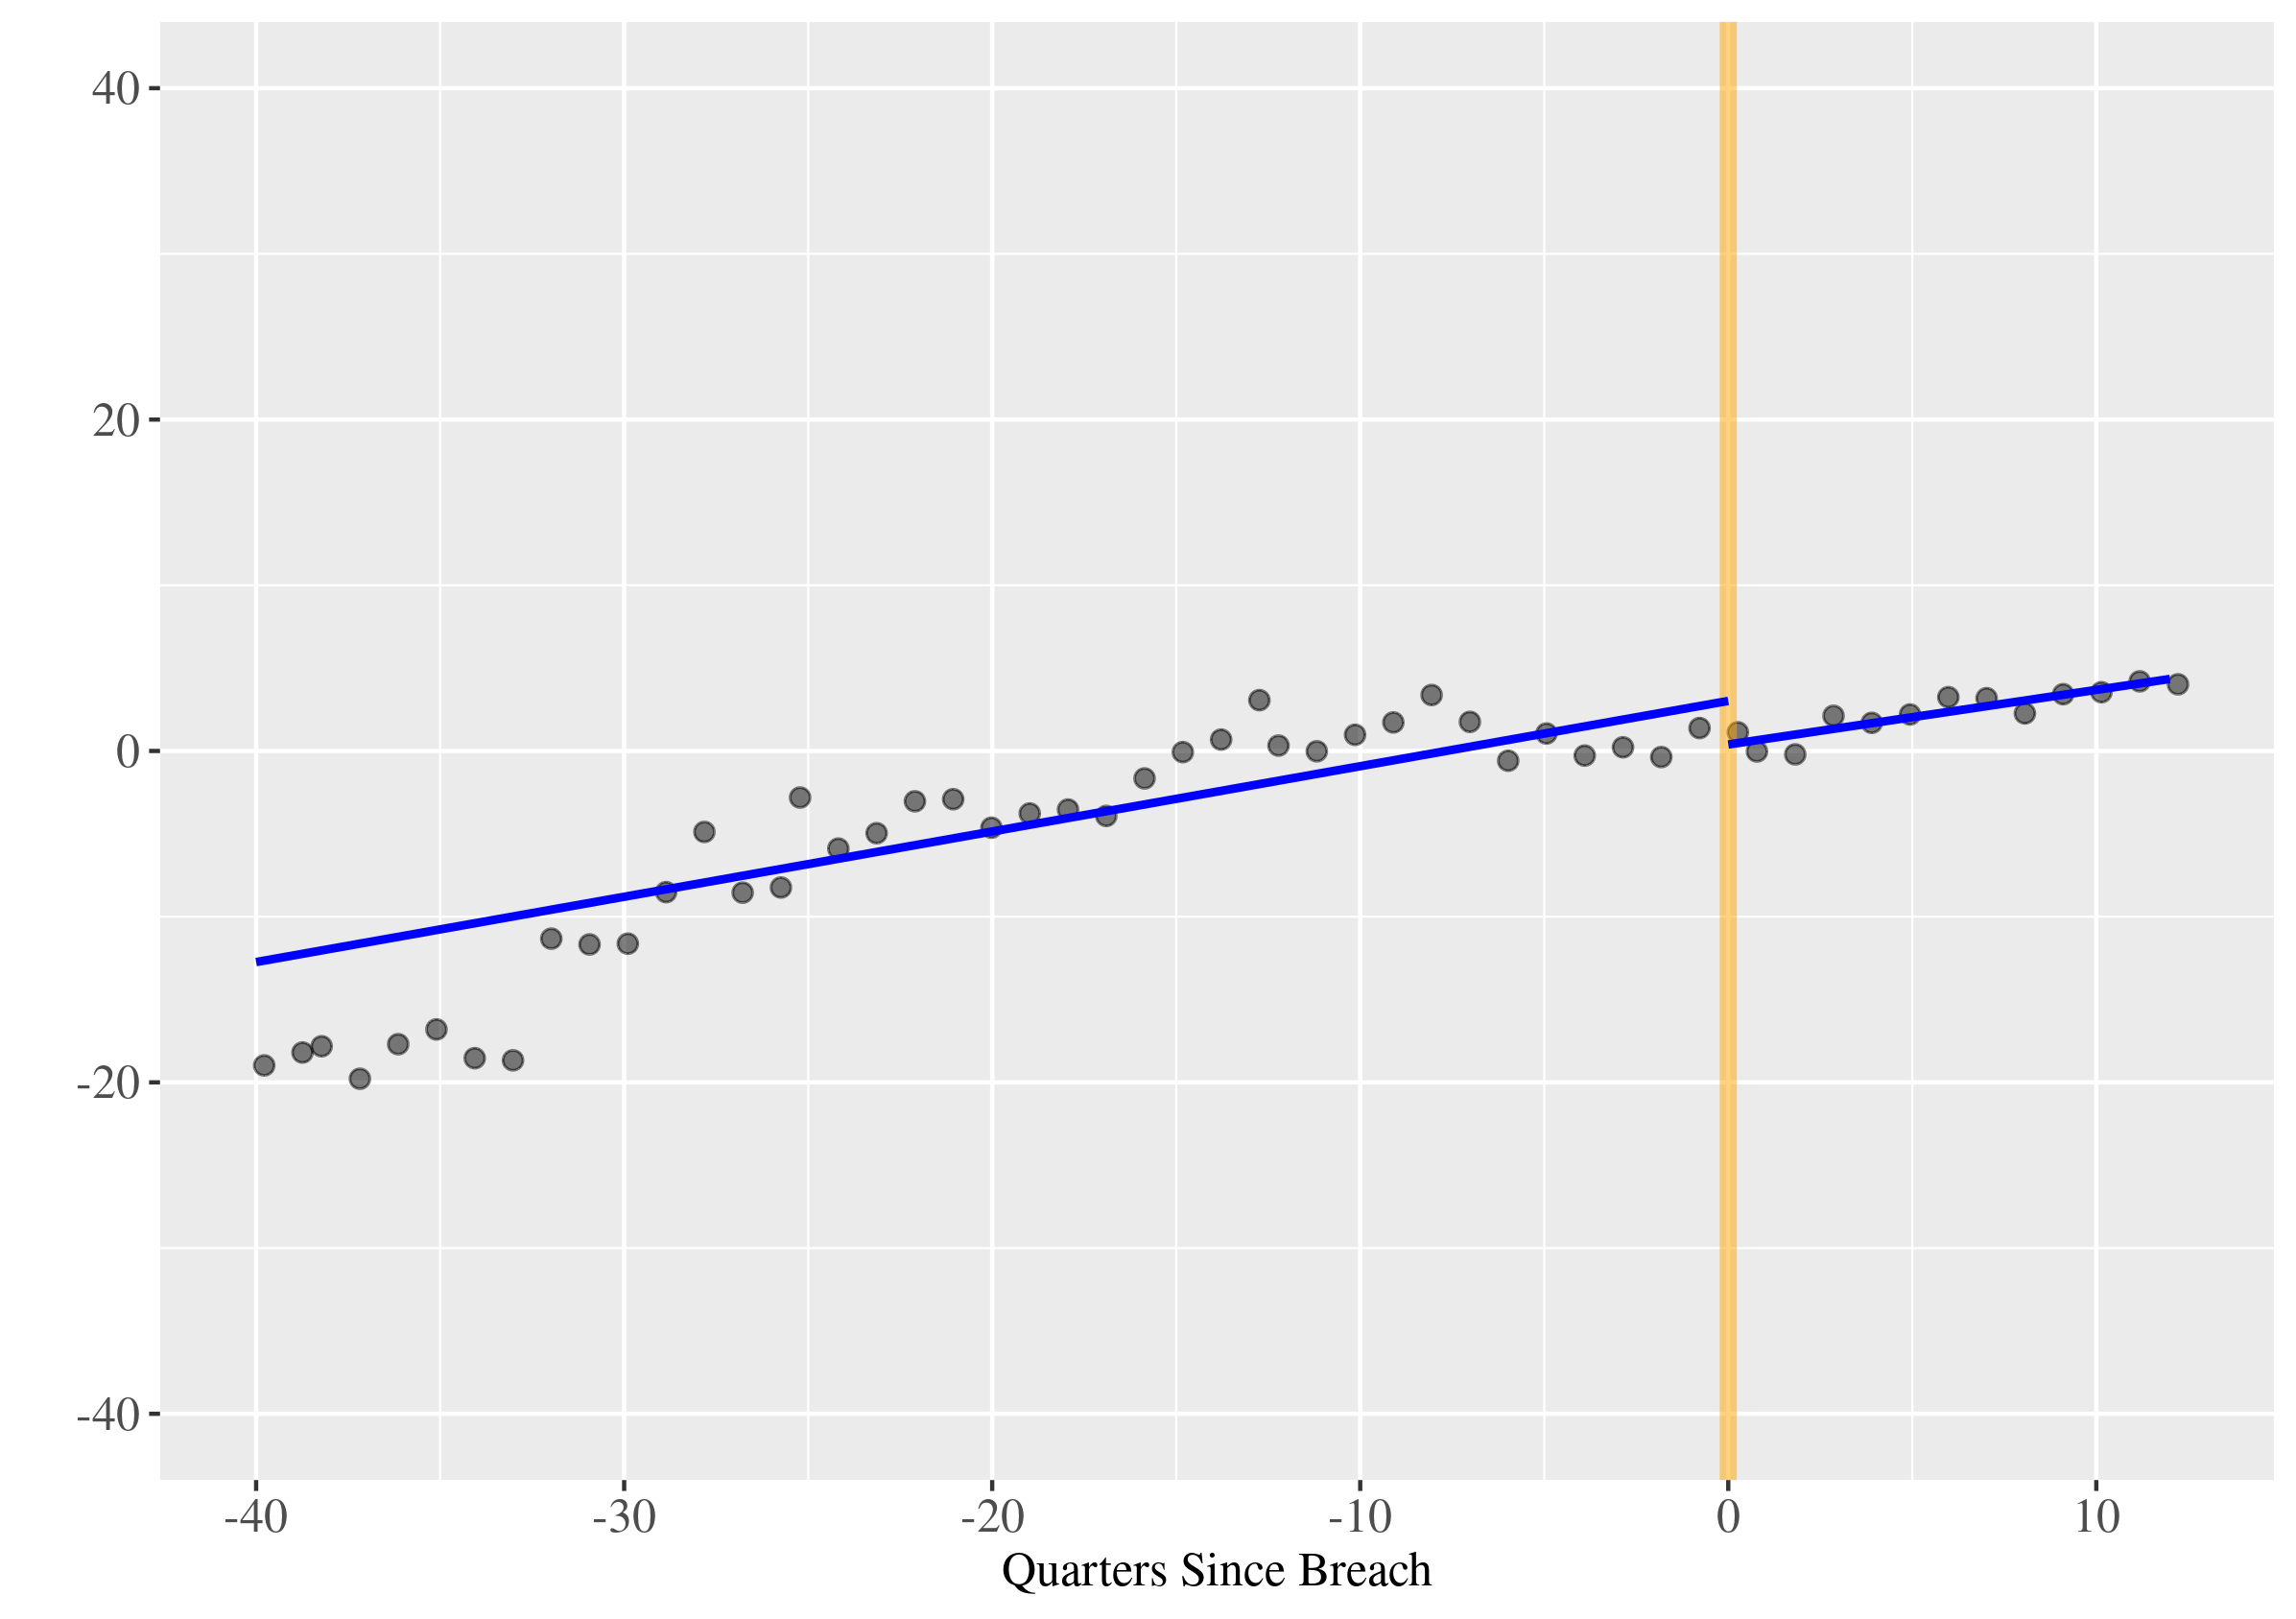
\includegraphics[width=\textwidth]{Images/mean_resid_nopiq_3y.png}
\end{figure}

\FloatBarrier
\clearpage

\subsection{Operating Expenses}

% Table created by stargazer v.5.2.2 by Marek Hlavac, Harvard University. E-mail: hlavac at fas.harvard.edu
% Date and time: Wed, Mar 27, 2019 - 04:32:17 PM
\begin{table}[!htbp] \centering 
  \caption{Operating expenses: main specification and controls} 
  \label{xopr1} 
\resizebox{\textwidth}{!}{\begin{tabular}{@{\extracolsep{5pt}}lccccc} 
\\[-1.8ex]\hline 
\hline \\[-1.8ex] 
 & \multicolumn{5}{c}{\textit{Dependent variable:}} \\ 
\cline{2-6} 
\\[-1.8ex] & \multicolumn{5}{c}{Operating Expenses} \\ 
\\[-1.8ex] & (1) & (2) & (3) & (4) & (5)\\ 
\hline \\[-1.8ex] 
 After Breach & 57.473 & $-$709.532 & $-$1,044.119$^{*}$ & 290.304 & $-$37.672 \\ 
  & (197.373) & (463.608) & (553.269) & (642.460) & (392.606) \\ 
  & & & & & \\ 
 After Breach x Quarter &  & 29.528$^{*}$ & 34.846$^{**}$ & 30.933$^{**}$ & 29.259$^{*}$ \\ 
  &  & (15.240) & (17.650) & (15.483) & (15.491) \\ 
  & & & & & \\ 
 Records Leaked (log) x After Breach &  &  & 31.075 &  &  \\ 
  &  &  & (19.970) &  &  \\ 
  & & & & & \\ 
 Google Search Index &  &  & 12.429$^{*}$ &  &  \\ 
  &  &  & (6.904) &  &  \\ 
  & & & & & \\ 
 Google Search Index x After Breach &  &  & 7.622 &  &  \\ 
  &  &  & (6.637) &  &  \\ 
  & & & & & \\ 
 After x Revenue Quartile 1 &  &  &  & $-$1,700.488$^{***}$ &  \\ 
  &  &  &  & (562.244) &  \\ 
  & & & & & \\ 
 After x Revenue Quartile 2 &  &  &  & $-$1,330.164$^{**}$ &  \\ 
  &  &  &  & (566.521) &  \\ 
  & & & & & \\ 
 After x Revenue Quartile 3 &  &  &  & $-$1,161.428$^{**}$ &  \\ 
  &  &  &  & (548.598) &  \\ 
  & & & & & \\ 
 Customer Data Leaked x After breach &  &  &  &  & $-$797.924$^{***}$ \\ 
  &  &  &  &  & (306.535) \\ 
  & & & & & \\ 
 Credit Card Leaked x After breach &  &  &  &  & $-$78.503 \\ 
  &  &  &  &  & (242.769) \\ 
  & & & & & \\ 
 SSN Leaked x After breach &  &  &  &  & $-$485.310 \\ 
  &  &  &  &  & (306.365) \\ 
  & & & & & \\ 
 Name Leaked x After breach &  &  &  &  & $-$482.602 \\ 
  &  &  &  &  & (316.239) \\ 
  & & & & & \\ 
 Address Leaked x After breach &  &  &  &  & 618.402$^{**}$ \\ 
  &  &  &  &  & (246.422) \\ 
  & & & & & \\ 
\hline \\[-1.8ex] 
Dependent Mean & 4214.72 & 4214.72 & 4214.72 & 4214.72 & 4214.72 \\ 
Dependent SD & 10047.91 & 10047.91 & 10047.91 & 10047.91 & 10047.91 \\ 
Observations & 11,899 & 11,899 & 11,309 & 11,899 & 11,899 \\ 
R$^{2}$ & 0.945 & 0.946 & 0.946 & 0.946 & 0.946 \\ 
Adjusted R$^{2}$ & 0.943 & 0.943 & 0.943 & 0.944 & 0.944 \\ 
\hline 
\hline \\[-1.8ex] 
\textit{Note:}  & \multicolumn{5}{r}{$^{*}$p$<$0.1; $^{**}$p$<$0.05; $^{***}$p$<$0.01} \\ 
 & \multicolumn{5}{r}{Standard errors clustered at the company level} \\ 
 & \multicolumn{5}{r}{Company and quarter fixed effects in all specifications} \\ 
 & \multicolumn{5}{r}{Prediction period is up to 10 years before breach, and event period up to 1 year after} \\ 
\end{tabular}} 
\end{table} 


% Table created by stargazer v.5.2.2 by Marek Hlavac, Harvard University. E-mail: hlavac at fas.harvard.edu
% Date and time: Wed, Mar 27, 2019 - 04:32:14 PM
\begin{table}[!htbp] \centering 
  \caption{Operating expenses: various event period lengths (robustness check)} 
  \label{xopr2} 
\resizebox{\textwidth}{!}{\begin{tabular}{@{\extracolsep{5pt}}lcccc} 
\\[-1.8ex]\hline 
\hline \\[-1.8ex] 
 & \multicolumn{4}{c}{\textit{Dependent variable:}} \\ 
\cline{2-5} 
\\[-1.8ex] & \multicolumn{4}{c}{Operating Expenses (Event Period)} \\ 
 & (6 Months) & (1 Year) & (2 Years) & (3 Years) \\ 
\hline \\[-1.8ex] 
 After Breach & $-$641.238 & $-$709.532 & $-$684.455 & $-$611.873 \\ 
  & (429.111) & (463.608) & (483.710) & (486.512) \\ 
  & & & & \\ 
 After Breach x Quarter & 30.817$^{**}$ & 29.528$^{*}$ & 25.035 & 21.037 \\ 
  & (14.763) & (15.240) & (15.687) & (15.651) \\ 
  & & & & \\ 
\hline \\[-1.8ex] 
Dependent Mean & 4214.72 & 4214.72 & 4214.72 & 4214.72 \\ 
Dependent SD & 10047.91 & 10047.91 & 10047.91 & 10047.91 \\ 
Observations & 10,820 & 11,899 & 13,686 & 15,190 \\ 
R$^{2}$ & 0.946 & 0.946 & 0.943 & 0.939 \\ 
Adjusted R$^{2}$ & 0.944 & 0.943 & 0.941 & 0.937 \\ 
\hline 
\hline \\[-1.8ex] 
\textit{Note:}  & \multicolumn{4}{r}{$^{*}$p$<$0.1; $^{**}$p$<$0.05; $^{***}$p$<$0.01} \\ 
 & \multicolumn{4}{r}{Standard errors clustered at the company level} \\ 
 & \multicolumn{4}{r}{Company and quarter fixed effects in all specifications} \\ 
\end{tabular}} 
\end{table} 


% Table created by stargazer v.5.2.2 by Marek Hlavac, Harvard University. E-mail: hlavac at fas.harvard.edu
% Date and time: Wed, Mar 27, 2019 - 05:16:14 PM
\begin{table}[!htbp] \centering 
  \caption{Operating expenses: first data breaches for each firm (robustness check)} 
  \label{xopr3} 
\resizebox{\textwidth}{!}{\begin{tabular}{@{\extracolsep{5pt}}lcccc} 
\\[-1.8ex]\hline 
\hline \\[-1.8ex] 
 & \multicolumn{4}{c}{\textit{Dependent variable:}} \\ 
\cline{2-5} 
\\[-1.8ex] & \multicolumn{4}{c}{Operating Expenses (Event Period)} \\ 
 & (6 Months) & (1 Year) & (2 Years) & (3 Years) \\ 
\hline \\[-1.8ex] 
 After Breach & $-$395.290 & $-$409.098 & $-$419.899$^{*}$ & $-$319.190 \\ 
  & (269.070) & (264.033) & (242.161) & (238.595) \\ 
  & & & & \\ 
 After Breach x Quarter & 15.983$^{**}$ & 17.202$^{**}$ & 17.924$^{**}$ & 14.280$^{*}$ \\ 
  & (8.095) & (8.141) & (7.647) & (8.051) \\ 
  & & & & \\ 
\hline \\[-1.8ex] 
Dependent Mean & 2443.43 & 2480.56 & 2525.9 & 2506.17 \\ 
Dependent SD & 6840.51 & 6967.15 & 7280.56 & 7399.64 \\ 
Observations & 8,350 & 9,019 & 10,207 & 11,229 \\ 
R$^{2}$ & 0.951 & 0.950 & 0.951 & 0.942 \\ 
Adjusted R$^{2}$ & 0.948 & 0.948 & 0.949 & 0.939 \\ 
\hline 
\hline \\[-1.8ex] 
\textit{Note:}  & \multicolumn{4}{r}{$^{*}$p$<$0.1; $^{**}$p$<$0.05; $^{***}$p$<$0.01} \\ 
 & \multicolumn{4}{r}{Standard errors clustered at the company level} \\ 
 & \multicolumn{4}{r}{Company and quarter fixed effects in all specifications} \\ 
\end{tabular}} 
\end{table} 


% Table created by stargazer v.5.2.2 by Marek Hlavac, Harvard University. E-mail: hlavac at fas.harvard.edu
% Date and time: Thu, Mar 28, 2019 - 05:46:27 PM
\begin{table}[!htbp] \centering 
  \caption{Operating expenses: breakdown by number of data breaches a firm has} 
  \label{xopr4} 
\resizebox{\textwidth}{!}{\begin{tabular}{@{\extracolsep{5pt}}lcccc} 
\\[-1.8ex]\hline 
\hline \\[-1.8ex] 
 & \multicolumn{4}{c}{\textit{Dependent variable:}} \\ 
\cline{2-5} 
\\[-1.8ex] & \multicolumn{4}{c}{Operating Expenses (Number of Breaches for Firm)} \\ 
 & (1) & (2) & (3) & (4+) \\ 
\hline \\[-1.8ex] 
 After Breach & $-$115.905 & 13.270 & $-$298.018 & $-$925.356 \\ 
  & (135.296) & (719.891) & (342.430) & (1,439.271) \\ 
  & & & & \\ 
 After Breach x Quarter & 8.364 & $-$10.026 & 18.026$^{*}$ & 70.763 \\ 
  & (5.631) & (20.137) & (9.306) & (45.528) \\ 
  & & & & \\ 
\hline \\[-1.8ex] 
Number of Data Breaches  & 255 & 158 & 85 & 210 \\ 
Dependent Mean & 1487.61 & 5293.86 & 4243.98 & 12907.84 \\ 
Dependent SD & 5034.45 & 11605.58 & 4796.78 & 16230.26 \\ 
Observations & 6,533 & 2,726 & 1,050 & 1,590 \\ 
R$^{2}$ & 0.951 & 0.943 & 0.951 & 0.930 \\ 
Adjusted R$^{2}$ & 0.948 & 0.940 & 0.947 & 0.925 \\ 
\hline 
\hline \\[-1.8ex] 
\textit{Note:}  & \multicolumn{4}{r}{$^{*}$p$<$0.1; $^{**}$p$<$0.05; $^{***}$p$<$0.01} \\ 
 & \multicolumn{4}{r}{Standard errors clustered at the company level} \\ 
 & \multicolumn{4}{r}{Company and quarter fixed effects in all specifications} \\ 
 & \multicolumn{4}{r}{Prediction period is up to 10 years before breach, and event period up to 1 year after} \\ 
\end{tabular}} 
\end{table} 

% Table created by stargazer v.5.2.2 by Marek Hlavac, Harvard University. E-mail: hlavac at fas.harvard.edu
% Date and time: Wed, Mar 27, 2019 - 04:10:53 PM
\begin{table}[!htbp] \centering 
  \caption{Operating Expenses: Offset event dates (robustness check)} 
  \label{xopr5} 
\resizebox{\textwidth}{!}{\begin{tabular}{@{\extracolsep{5pt}}lccccc} 
\\[-1.8ex]\hline 
\hline \\[-1.8ex] 
 & \multicolumn{5}{c}{\textit{Dependent variable:}} \\ 
\cline{2-6} 
\\[-1.8ex] & \multicolumn{5}{c}{Operating Expenses (Offset of Event Date)} \\ 
 & (0) & (-2 Years) & (-3 Years) & (+2 Years) & (+3 Years) \\ 
\hline \\[-1.8ex] 
 After Breach & $-$684.455 & $-$407.196 & $-$424.522 & $-$687.913 & $-$964.997$^{**}$ \\ 
  & (483.710) & (327.361) & (648.659) & (482.451) & (414.988) \\ 
  & & & & & \\ 
 After Breach x Quarter & 25.035 & 16.132 & 20.579 & 15.328 & 19.619 \\ 
  & (15.687) & (12.365) & (27.597) & (16.063) & (13.684) \\ 
  & & & & & \\ 
\hline \\[-1.8ex] 
Dependent Mean & 4214.72 & 4214.72 & 4214.72 & 4214.72 & 4214.72 \\ 
Dependent SD & 10047.91 & 10047.91 & 10047.91 & 10047.91 & 10047.91 \\ 
Observations & 13,686 & 6,836 & 5,016 & 15,190 & 16,471 \\ 
R$^{2}$ & 0.943 & 0.956 & 0.955 & 0.939 & 0.939 \\ 
Adjusted R$^{2}$ & 0.941 & 0.953 & 0.951 & 0.937 & 0.937 \\ 
\hline 
\hline \\[-1.8ex] 
\textit{Note:}  & \multicolumn{5}{r}{$^{*}$p$<$0.1; $^{**}$p$<$0.05; $^{***}$p$<$0.01} \\ 
 & \multicolumn{5}{r}{Standard errors clustered at the company level} \\ 
 & \multicolumn{5}{r}{Company and quarter fixed effects in all specifications} \\ 
 & \multicolumn{5}{r}{Prediction period is up to 10 years before breach, and event period up to 1 year after} \\ 
\end{tabular}} 
\end{table} 

\FloatBarrier

\begin{figure}
    \centering
    \caption{Mean residual operating expenses (fixed effects removed)}
    \label{xoprfig}
    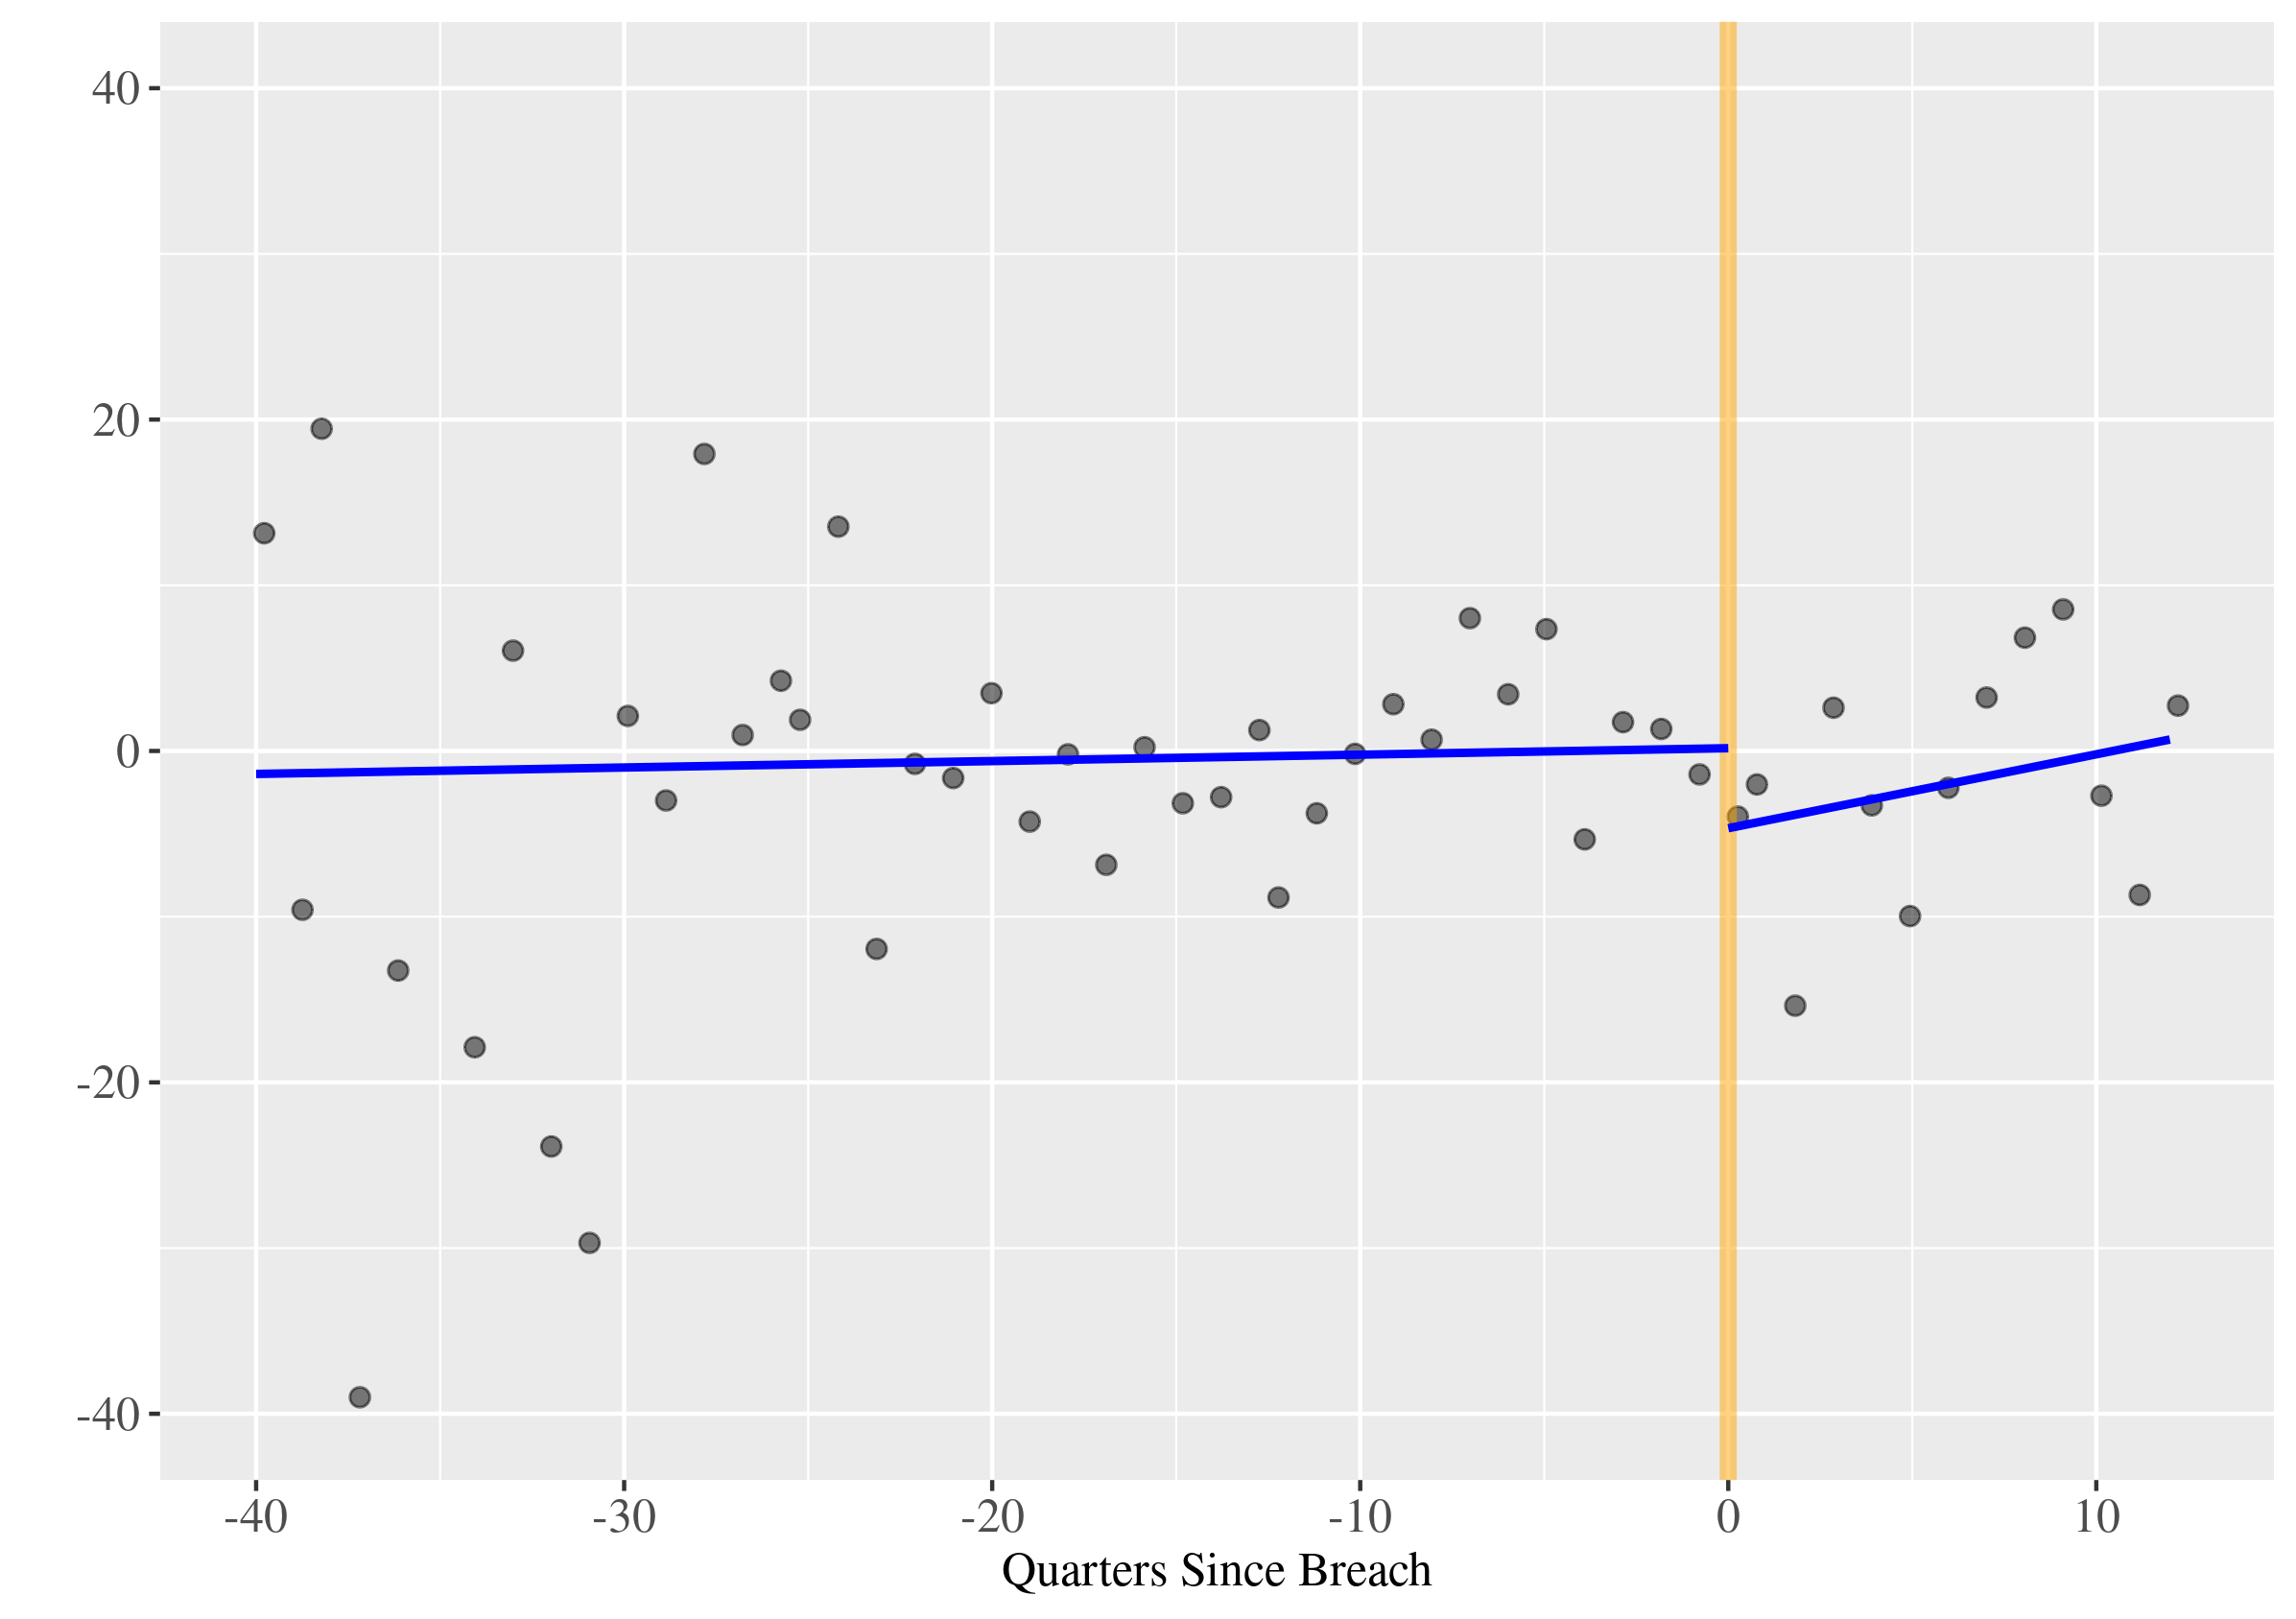
\includegraphics[width=\textwidth]{Images/mean_resid_xoprq_3y.png}
\end{figure}

\FloatBarrier
\clearpage

\subsection{Net Income}

% Table created by stargazer v.5.2.2 by Marek Hlavac, Harvard University. E-mail: hlavac at fas.harvard.edu
% Date and time: Tue, Mar 26, 2019 - 06:06:56 PM
\begin{table}[!htbp] \centering 
  \caption{Net income: main specification and controls} 
  \label{pr1} 
\resizebox{\textwidth}{!}{\begin{tabular}{@{\extracolsep{5pt}}lccccc} 
\\[-1.8ex]\hline 
\hline \\[-1.8ex] 
 & \multicolumn{5}{c}{\textit{Dependent variable:}} \\ 
\cline{2-6} 
\\[-1.8ex] & \multicolumn{5}{c}{Net Income} \\ 
\\[-1.8ex] & (1) & (2) & (3) & (4) & (5)\\ 
\hline \\[-1.8ex] 
 After Breach & $-$86.377 & $-$390.372$^{**}$ & $-$453.561$^{**}$ & $-$383.633 & $-$94.755 \\ 
  & (66.703) & (171.958) & (206.152) & (290.527) & (146.636) \\ 
  & & & & & \\ 
 After Breach x Quarter &  & 11.697$^{**}$ & 12.728$^{**}$ & 11.893$^{**}$ & 11.997$^{**}$ \\ 
  &  & (4.871) & (5.103) & (4.850) & (4.842) \\ 
  & & & & & \\ 
 Records Leaked (log) x After Breach &  &  & 2.999 &  &  \\ 
  &  &  & (5.099) &  &  \\ 
  & & & & & \\ 
 Google Search Index &  &  & $-$1.874 &  &  \\ 
  &  &  & (1.954) &  &  \\ 
  & & & & & \\ 
 Google Search Index x After Breach &  &  & 1.279 &  &  \\ 
  &  &  & (2.623) &  &  \\ 
  & & & & & \\ 
 After x Revenue Quartile 1 &  &  &  & $-$83.509 &  \\ 
  &  &  &  & (226.990) &  \\ 
  & & & & & \\ 
 After x Revenue Quartile 2 &  &  &  & 16.797 &  \\ 
  &  &  &  & (217.332) &  \\ 
  & & & & & \\ 
 After x Revenue Quartile 3 &  &  &  & 49.027 &  \\ 
  &  &  &  & (214.735) &  \\ 
  & & & & & \\ 
 Customer Data Leaked x After breach &  &  &  &  & $-$362.903$^{***}$ \\ 
  &  &  &  &  & (100.321) \\ 
  & & & & & \\ 
 Credit Card Leaked x After breach &  &  &  &  & 75.753 \\ 
  &  &  &  &  & (99.050) \\ 
  & & & & & \\ 
 SSN Leaked x After breach &  &  &  &  & $-$247.812$^{**}$ \\ 
  &  &  &  &  & (115.114) \\ 
  & & & & & \\ 
 Name Leaked x After breach &  &  &  &  & 10.909 \\ 
  &  &  &  &  & (83.450) \\ 
  & & & & & \\ 
 Address Leaked x After breach &  &  &  &  & $-$91.312 \\ 
  &  &  &  &  & (75.771) \\ 
  & & & & & \\ 
\hline \\[-1.8ex] 
Dependent Mean & 427.34 & 427.34 & 427.34 & 427.34 & 427.34 \\ 
Dependent SD & 1816.55 & 1816.55 & 1816.55 & 1816.55 & 1816.55 \\ 
Observations & 11,952 & 11,952 & 11,359 & 11,952 & 11,952 \\ 
R$^{2}$ & 0.290 & 0.291 & 0.288 & 0.291 & 0.294 \\ 
Adjusted R$^{2}$ & 0.262 & 0.263 & 0.259 & 0.262 & 0.265 \\ 
\hline 
\hline \\[-1.8ex] 
\textit{Note:}  & \multicolumn{5}{r}{$^{*}$p$<$0.1; $^{**}$p$<$0.05; $^{***}$p$<$0.01} \\ 
 & \multicolumn{5}{r}{Standard errors clustered at the company level} \\ 
 & \multicolumn{5}{r}{Company and quarter fixed effects in all specifications} \\ 
 & \multicolumn{5}{r}{Prediction period is up to 10 years before breach, and event period up to 1 year after} \\ 
\end{tabular}} 
\end{table} 

% Table created by stargazer v.5.2.2 by Marek Hlavac, Harvard University. E-mail: hlavac at fas.harvard.edu
% Date and time: Tue, Mar 26, 2019 - 06:06:57 PM
\begin{table}[!htbp] \centering 
  \caption{Net income: various event period lengths (robustness check)} 
  \label{pr2} 
\resizebox{\textwidth}{!}{\begin{tabular}{@{\extracolsep{5pt}}lcccc} 
\\[-1.8ex]\hline 
\hline \\[-1.8ex] 
 & \multicolumn{4}{c}{\textit{Dependent variable:}} \\ 
\cline{2-5} 
\\[-1.8ex] & \multicolumn{4}{c}{Net Income (Event Period)} \\ 
 & (6 Months) & (1 Year) & (2 Years) & (3 Years) \\ 
 \hline \\[-1.8ex] 
 After Breach & $-$371.171$^{*}$ & $-$390.372$^{**}$ & $-$410.271$^{**}$ & $-$422.288$^{**}$ \\ 
  & (192.567) & (171.958) & (169.343) & (165.827) \\ 
  & & & & \\ 
 After Breach x Quarter & 12.304$^{**}$ & 11.697$^{**}$ & 11.839$^{**}$ & 11.604$^{***}$ \\ 
  & (5.570) & (4.871) & (4.649) & (4.446) \\ 
  & & & & \\ 
\hline \\[-1.8ex] 
Dependent Mean & 419.67 & 427.34 & 432.49 & 427.88 \\ 
Dependent SD & 1818.62 & 1816.55 & 1790.5 & 1839.08 \\ 
Observations & 10,862 & 11,952 & 13,743 & 15,247 \\ 
R$^{2}$ & 0.282 & 0.291 & 0.307 & 0.309 \\ 
Adjusted R$^{2}$ & 0.250 & 0.263 & 0.283 & 0.287 \\ 
\hline 
\hline \\[-1.8ex] 
\textit{Note:}  & \multicolumn{4}{r}{$^{*}$p$<$0.1; $^{**}$p$<$0.05; $^{***}$p$<$0.01} \\ 
 & \multicolumn{4}{r}{Standard errors clustered at the company level} \\ 
 & \multicolumn{4}{r}{Company and quarter fixed effects in all specifications} \\ 
\end{tabular}} 
\end{table} 


% Table created by stargazer v.5.2.2 by Marek Hlavac, Harvard University. E-mail: hlavac at fas.harvard.edu
% Date and time: Wed, Mar 27, 2019 - 05:25:11 PM
\begin{table}[!htbp] \centering 
  \caption{Net income: first data breaches for each firm (robustness check)} 
  \label{pr3} 
\resizebox{\textwidth}{!}{\begin{tabular}{@{\extracolsep{5pt}}lcccc} 
\\[-1.8ex]\hline 
\hline \\[-1.8ex] 
 & \multicolumn{4}{c}{\textit{Dependent variable:}} \\ 
\cline{2-5} 
\\[-1.8ex] & \multicolumn{4}{c}{Net Income (Event Period)} \\ 
 & (6 Months) & (1 Year) & (2 Years) & (3 Years) \\ 
\\[-1.8ex] & (1) & (2) & (3) & (4)\\ 
\hline \\[-1.8ex] 
 After Breach & $-$53.339 & $-$41.920 & $-$31.425 & $-$3.151 \\ 
  & (106.911) & (94.414) & (87.813) & (89.715) \\ 
  & & & & \\ 
 After Breach x Quarter & 1.726 & 1.490 & 1.333 & 0.157 \\ 
  & (2.702) & (2.448) & (2.298) & (2.533) \\ 
  & & & & \\ 
\hline \\[-1.8ex] 
Dependent Mean & 229.02 & 231.74 & 226.05 & 210.84 \\ 
Dependent SD & 914.37 & 925.65 & 946.25 & 1123.7 \\ 
Observations & 8,371 & 9,046 & 10,234 & 11,256 \\ 
R$^{2}$ & 0.579 & 0.585 & 0.540 & 0.400 \\ 
Adjusted R$^{2}$ & 0.555 & 0.562 & 0.517 & 0.374 \\ 
\hline 
\hline \\[-1.8ex] 
\textit{Note:}  & \multicolumn{4}{r}{$^{*}$p$<$0.1; $^{**}$p$<$0.05; $^{***}$p$<$0.01} \\ 
 & \multicolumn{4}{r}{Standard errors clustered at the company level} \\ 
 & \multicolumn{4}{r}{Company and quarter fixed effects in all specifications} \\ 
\end{tabular}} 
\end{table} 


% Table created by stargazer v.5.2.2 by Marek Hlavac, Harvard University. E-mail: hlavac at fas.harvard.edu
% Date and time: Thu, Mar 28, 2019 - 05:43:32 PM
\begin{table}[!htbp] \centering 
  \caption{Net income: breakdown by number of data breaches a firm has} 
  \label{pr4} 
\resizebox{\textwidth}{!}{\begin{tabular}{@{\extracolsep{5pt}}lcccc} 
\\[-1.8ex]\hline 
\hline \\[-1.8ex] 
 & \multicolumn{4}{c}{\textit{Dependent variable:}} \\ 
\cline{2-5} 
\\[-1.8ex] & \multicolumn{4}{c}{Net Income (Number of Breaches for Firm)} \\ 
 & (1) & (2) & (3) & (4+) \\ 
\hline \\[-1.8ex] 
 After Breach & $-$74.962 & $-$258.433 & 20.965 & $-$712.170 \\ 
  & (122.444) & (217.311) & (233.661) & (611.408) \\ 
  & & & & \\ 
 After Breach x Quarter & 2.261 & 6.755 & $-$0.261 & 22.401 \\ 
  & (3.132) & (5.614) & (7.770) & (16.178) \\ 
  & & & & \\ 
\hline \\[-1.8ex] 
Number of Data Breaches  & 255 & 158 & 85 & 210 \\ 
Dependent Mean & 109.83 & 443.13 & 544.93 & 1609.38 \\ 
Dependent SD & 680.93 & 1200.23 & 1157.95 & 4170.13 \\ 
Observations & 6,549 & 2,733 & 1,052 & 1,618 \\ 
R$^{2}$ & 0.347 & 0.657 & 0.400 & 0.196 \\ 
Adjusted R$^{2}$ & 0.314 & 0.640 & 0.348 & 0.150 \\ 
\hline 
\hline \\[-1.8ex] 
\textit{Note:}  & \multicolumn{4}{r}{$^{*}$p$<$0.1; $^{**}$p$<$0.05; $^{***}$p$<$0.01} \\ 
 & \multicolumn{4}{r}{Standard errors clustered at the company level} \\ 
 & \multicolumn{4}{r}{Company and quarter fixed effects in all specifications} \\ 
 & \multicolumn{4}{r}{Prediction period is up to 10 years before breach, and event period up to 1 year after} \\ 
\end{tabular}} 
\end{table} 


% Table created by stargazer v.5.2.2 by Marek Hlavac, Harvard University. E-mail: hlavac at fas.harvard.edu
% Date and time: Wed, Mar 27, 2019 - 04:10:52 PM
\begin{table}[!htbp] \centering 
  \caption{Net income: offset event dates (robustness check)} 
  \label{pr5} 
\resizebox{\textwidth}{!}{\begin{tabular}{@{\extracolsep{5pt}}lccccc} 
\\[-1.8ex]\hline 
\hline \\[-1.8ex] 
 & \multicolumn{5}{c}{\textit{Dependent variable:}} \\ 
\cline{2-6} 
\\[-1.8ex] & \multicolumn{5}{c}{Net Income (Offset of Event Date)} \\ 
 & (0) & (-2 Years) & (-3 Years) & (+2 Years) & (+3 Years) \\ 
\hline \\[-1.8ex] 
 After Breach & $-$390.372$^{**}$ & $-$136.829$^{*}$ & $-$103.339$^{*}$ & $-$574.147$^{*}$ & $-$336.764$^{*}$ \\ 
  & (171.958) & (76.415) & (53.155) & (294.070) & (200.623) \\ 
  & & & & & \\ 
 After Breach x Quarter & 11.697$^{**}$ & 4.395 & 4.208$^{*}$ & 15.567$^{**}$ & 8.819 \\ 
  & (4.871) & (2.784) & (2.327) & (7.746) & (6.164) \\ 
  & & & & & \\ 
\hline \\[-1.8ex] 
Dependent Mean & 427.34 & 427.34 & 427.34 & 427.34 & 427.34 \\ 
Dependent SD & 1816.55 & 1816.55 & 1816.55 & 1816.55 & 1816.55 \\ 
Observations & 11,952 & 6,852 & 5,029 & 15,247 & 16,533 \\ 
R$^{2}$ & 0.291 & 0.732 & 0.743 & 0.308 & 0.311 \\ 
Adjusted R$^{2}$ & 0.263 & 0.714 & 0.723 & 0.286 & 0.291 \\ 
\hline 
\hline \\[-1.8ex] 
\textit{Note:}  & \multicolumn{5}{r}{$^{*}$p$<$0.1; $^{**}$p$<$0.05; $^{***}$p$<$0.01} \\ 
 & \multicolumn{5}{r}{Standard errors clustered at the company level} \\ 
 & \multicolumn{5}{r}{Company and quarter fixed effects in all specifications} \\ 
 & \multicolumn{5}{r}{Prediction period is up to 10 years before breach, and event period up to 1 year after} \\ 
\end{tabular}} 
\end{table} 

\FloatBarrier
\clearpage

\begin{figure}
    \centering
    \caption{Mean residual profit (fixed effects removed)}
    \label{prfig}
    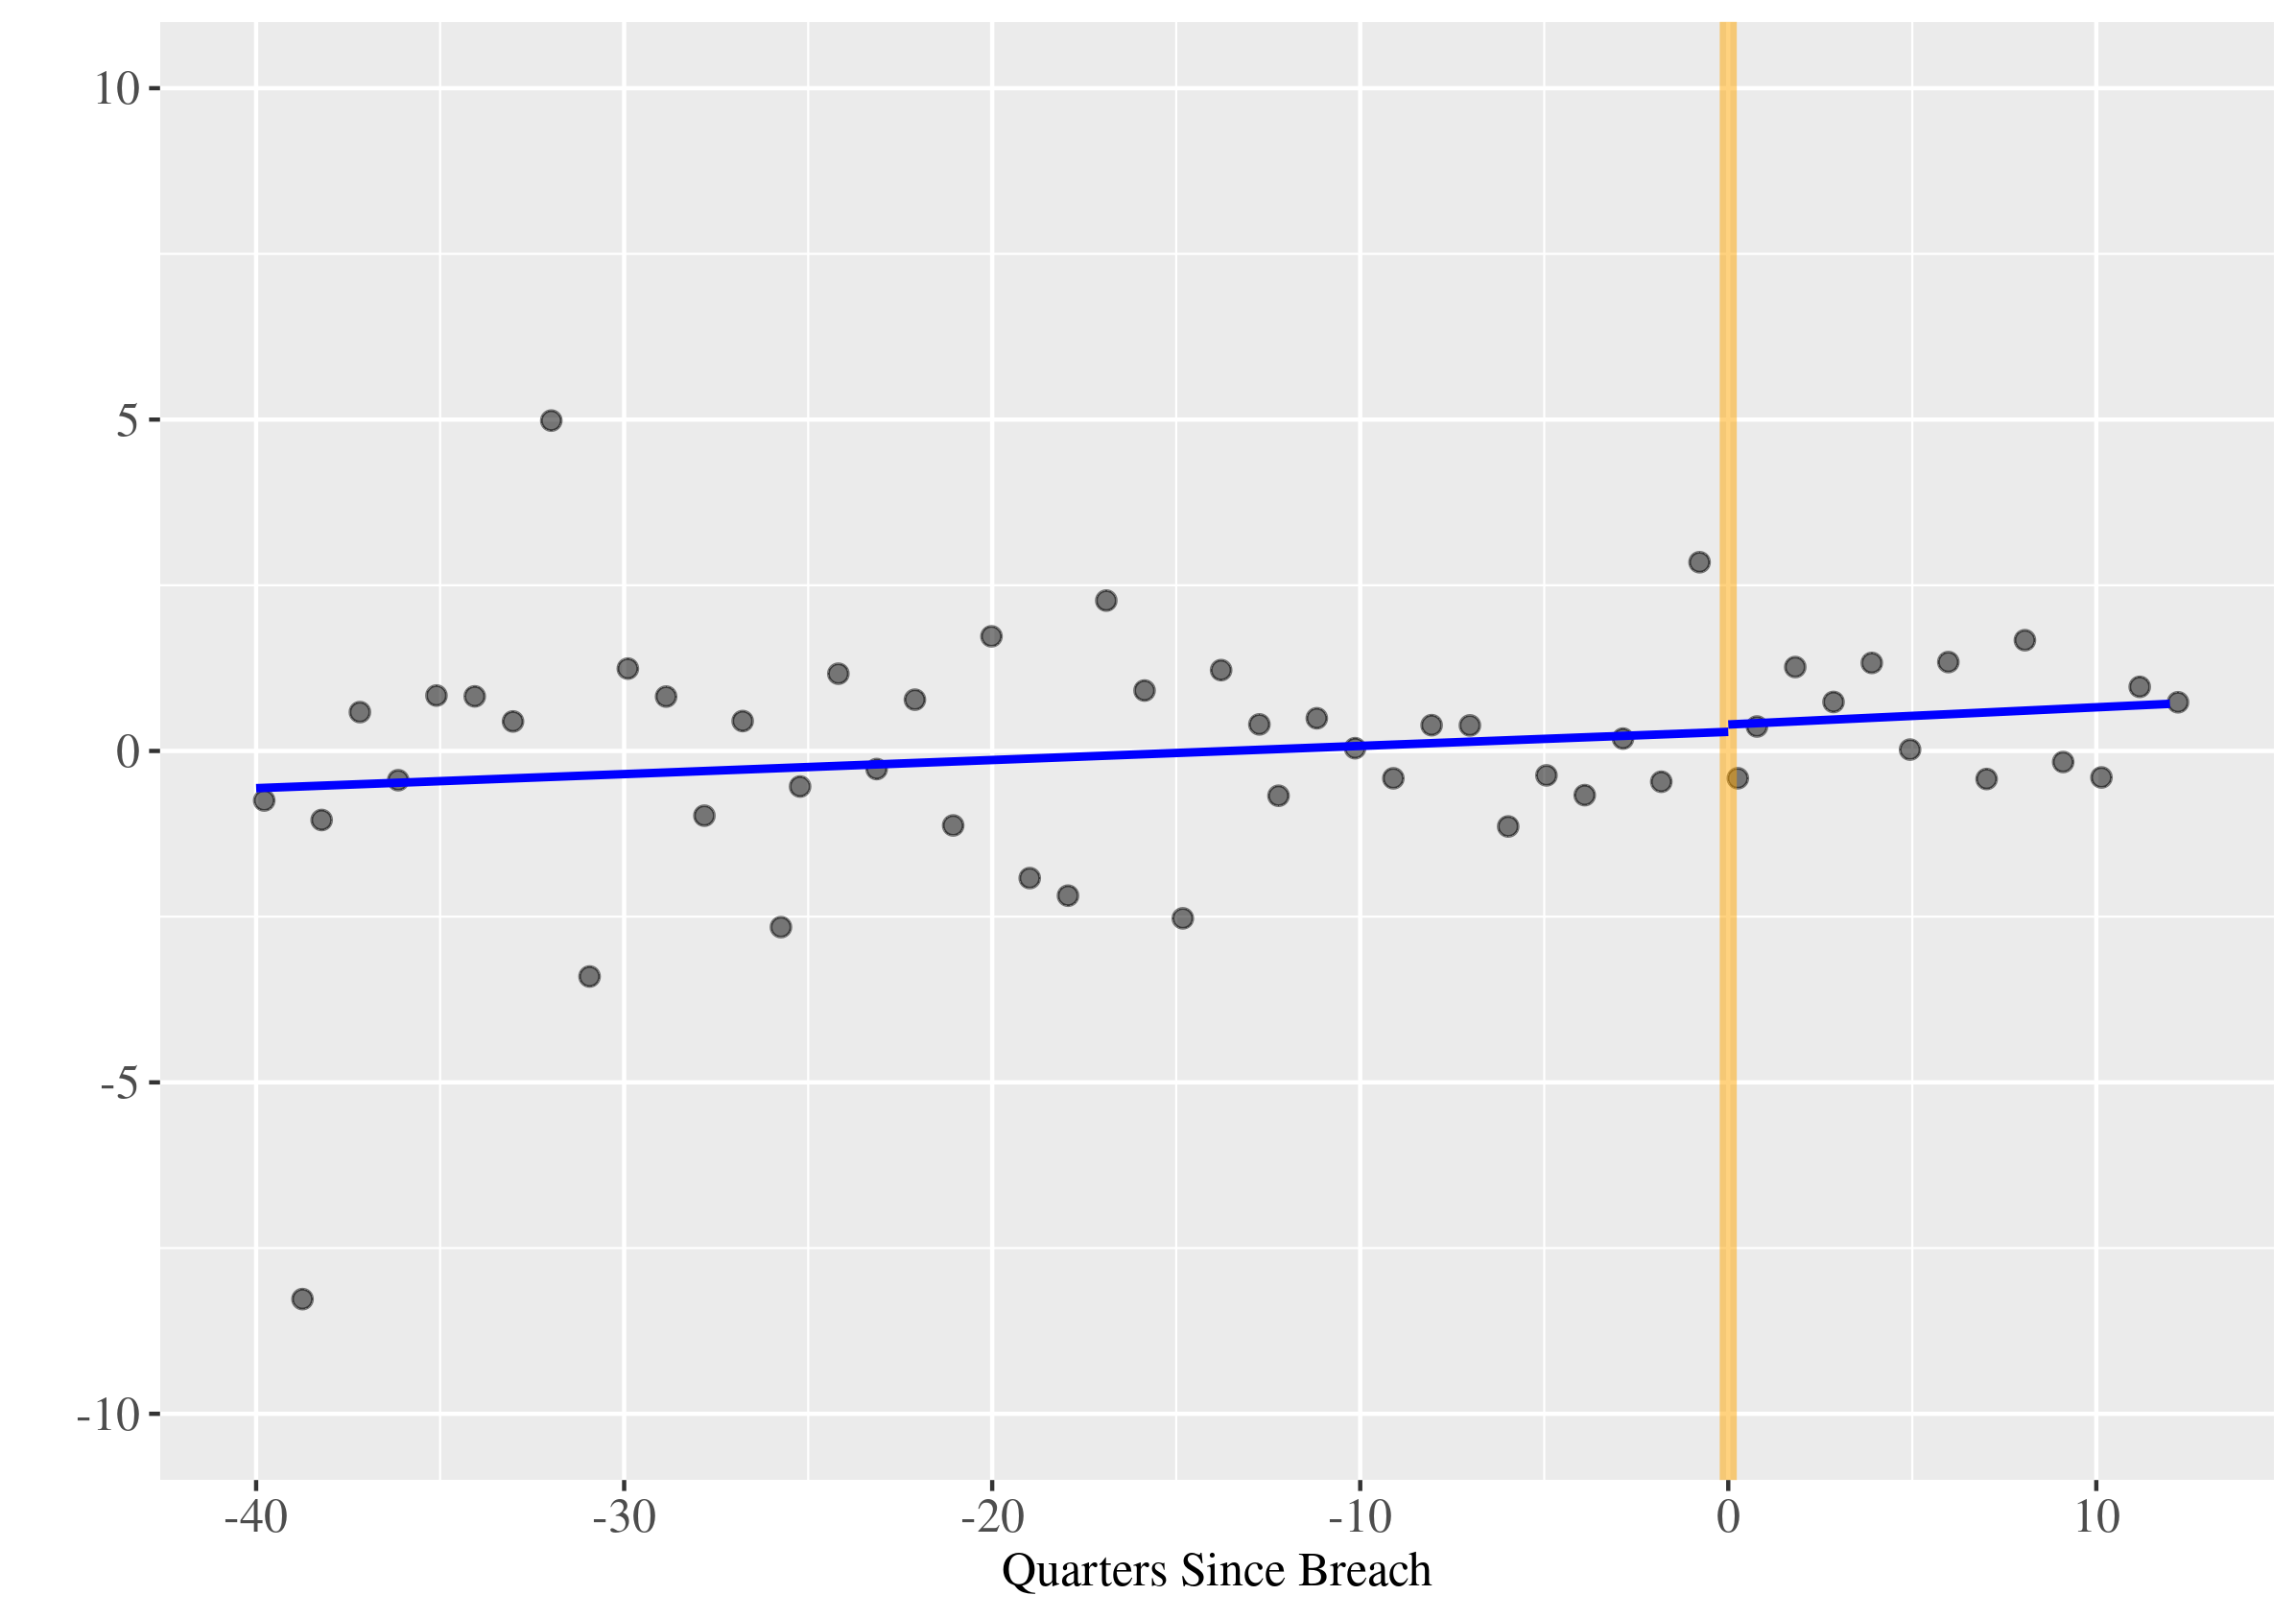
\includegraphics[width=\textwidth]{Images/mean_resid_profit_3y.png}
\end{figure}

\FloatBarrier
\clearpage

\subsection{Other Outcomes}



% Table created by stargazer v.5.2.2 by Marek Hlavac, Harvard University. E-mail: hlavac at fas.harvard.edu
% Date and time: Sun, Mar 31, 2019 - 08:27:56 PM
\begin{table}[!htbp] \centering 
  \caption{Other outcomes: main specification} 
  \label{otheroutcomes} 
\resizebox{\textwidth}{!}{\begin{tabular}{@{\extracolsep{5pt}}lcccccc} 
\\[-1.8ex]\hline 
\hline \\[-1.8ex] 
 & \multicolumn{6}{c}{\textit{Dependent variable:}} \\ 
\cline{2-7} 
\\[-1.8ex] & Sales, General and & Total Shareholders' & Earnings per & Number of & Google Searches & Google Searches \\ 
 & Other Expenses & Equity & Share (Basic) & Employees & (Company Name) & (Stock Ticker) \\ 
\\[-1.8ex] & (1) & (2) & (3) & (4) & (5) & (6)\\ 
\hline \\[-1.8ex] 
 After Breach & $-$426.048$^{***}$ & $-$6,758.839$^{**}$ & $-$6.142 & $-$2.253 & $-$2.136$^{*}$ & $-$1.610 \\ 
  & (157.999) & (2,672.161) & (5.979) & (6.006) & (1.171) & (1.162) \\ 
  & & & & & & \\ 
 After Breach x Quarters Since Breach & 14.497$^{***}$ & 223.119$^{***}$ & 0.121 & 0.153 & 0.052 & 0.029 \\ 
  & (5.098) & (81.262) & (0.115) & (0.188) & (0.039) & (0.040) \\ 
  & & & & & & \\ 
\hline \\[-1.8ex] 
Dependent Mean & 1045.61 & 14123.25 & 3.03  & 63.31 & 26.12 & 30.44 \\ 
Dependent SD & 2255.5 & 34818.35 & 72.91 & 154.54 & 27.84 & 28.34 \\ 
Observations & 9,430 & 11,914 & 11,771 & 6,357 & 11,401 & 11,866 \\ 
R$^{2}$ & 0.946 & 0.927 & 0.240 & 0.990 & 0.865 & 0.858 \\ 
Adjusted R$^{2}$ & 0.944 & 0.924 & 0.209 & 0.989 & 0.859 & 0.853 \\ 
\hline 
\hline \\[-1.8ex] 
\textit{Note:}  & \multicolumn{6}{r}{$^{*}$p$<$0.1; $^{**}$p$<$0.05; $^{***}$p$<$0.01} \\ 
 & \multicolumn{6}{r}{Standard Errors clustered at the quarter level} \\ 
 & \multicolumn{6}{r}{Company and quarter fixed effects in all specifications} \\ 
 & \multicolumn{6}{r}{Prediction period is up to 10 years before breach, and event period 1 year after} \\ 
\end{tabular}} 
\end{table} 

\clearpage
\FloatBarrier

\subsection{Stock Market}

\begin{figure}[!htbp]
    \centering
    \caption{Capital Asset Pricing Model stock market event study}
    \label{capmfig}
    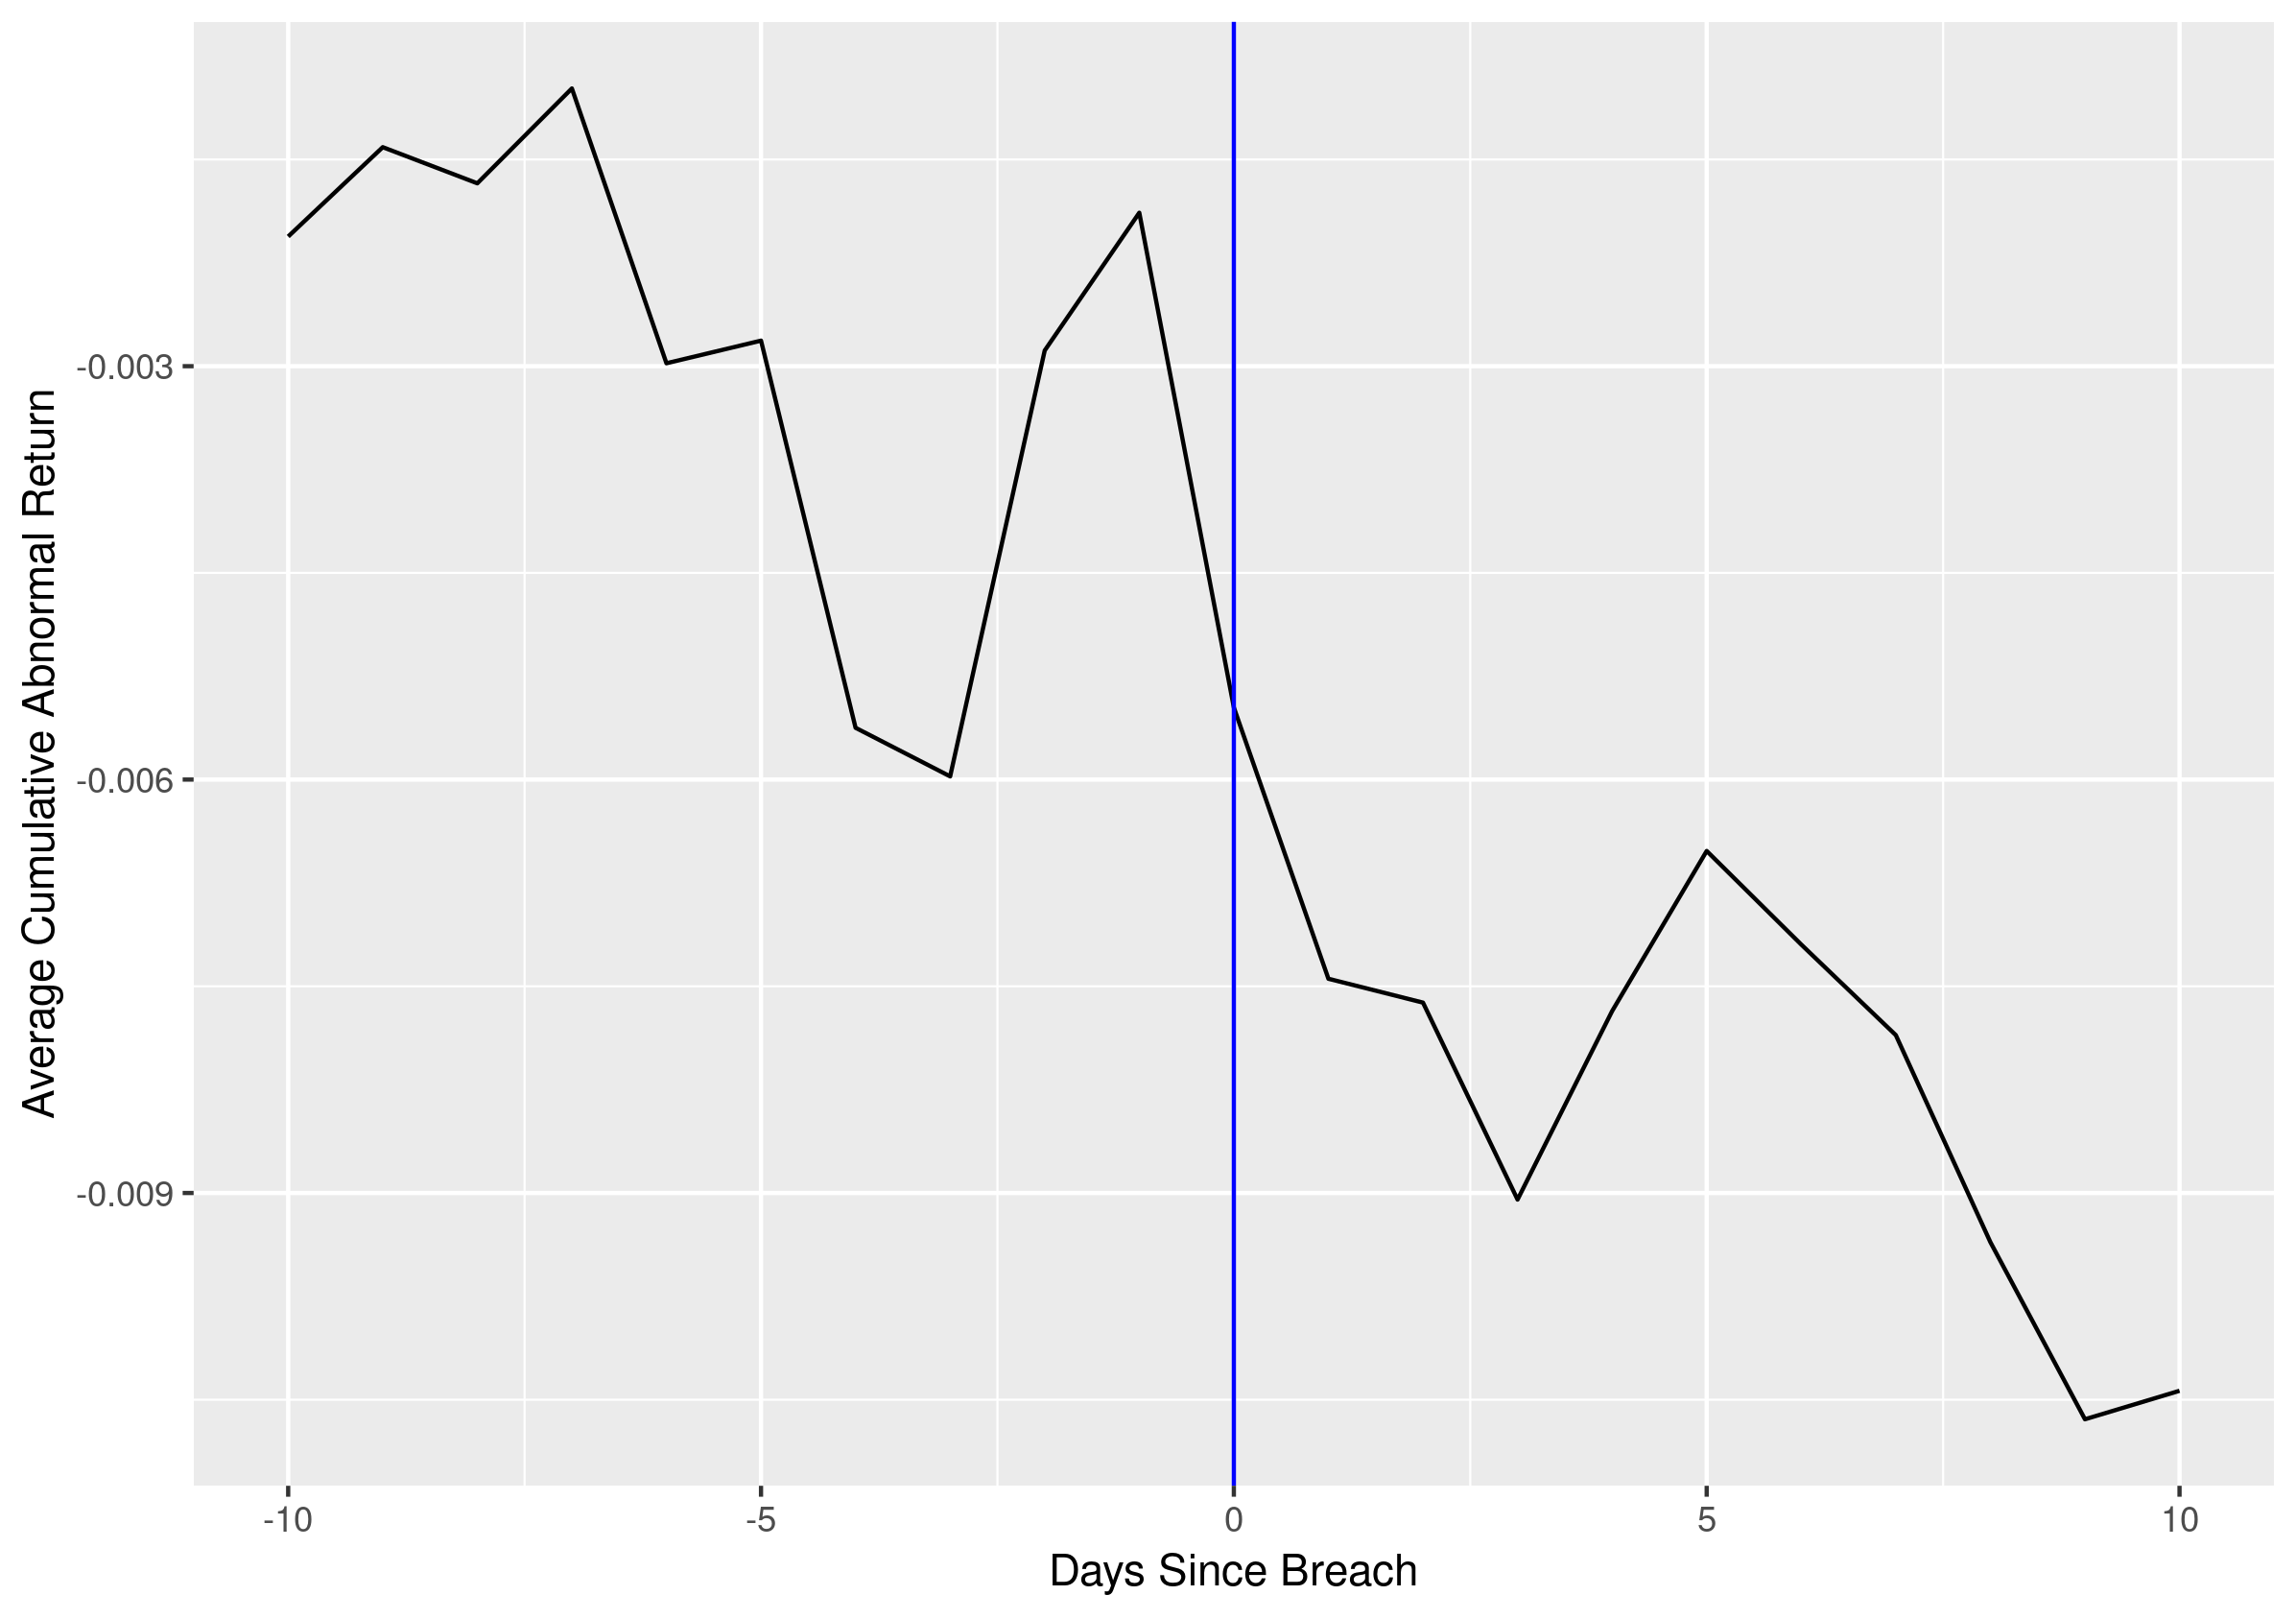
\includegraphics[width=\textwidth]{Images/mmodel_eventstudy.png}
\end{figure}

\FloatBarrier

\begin{figure}[!htbp]
    \centering
    \caption{Fama-French Model stock market event study}
    \label{fffig}
    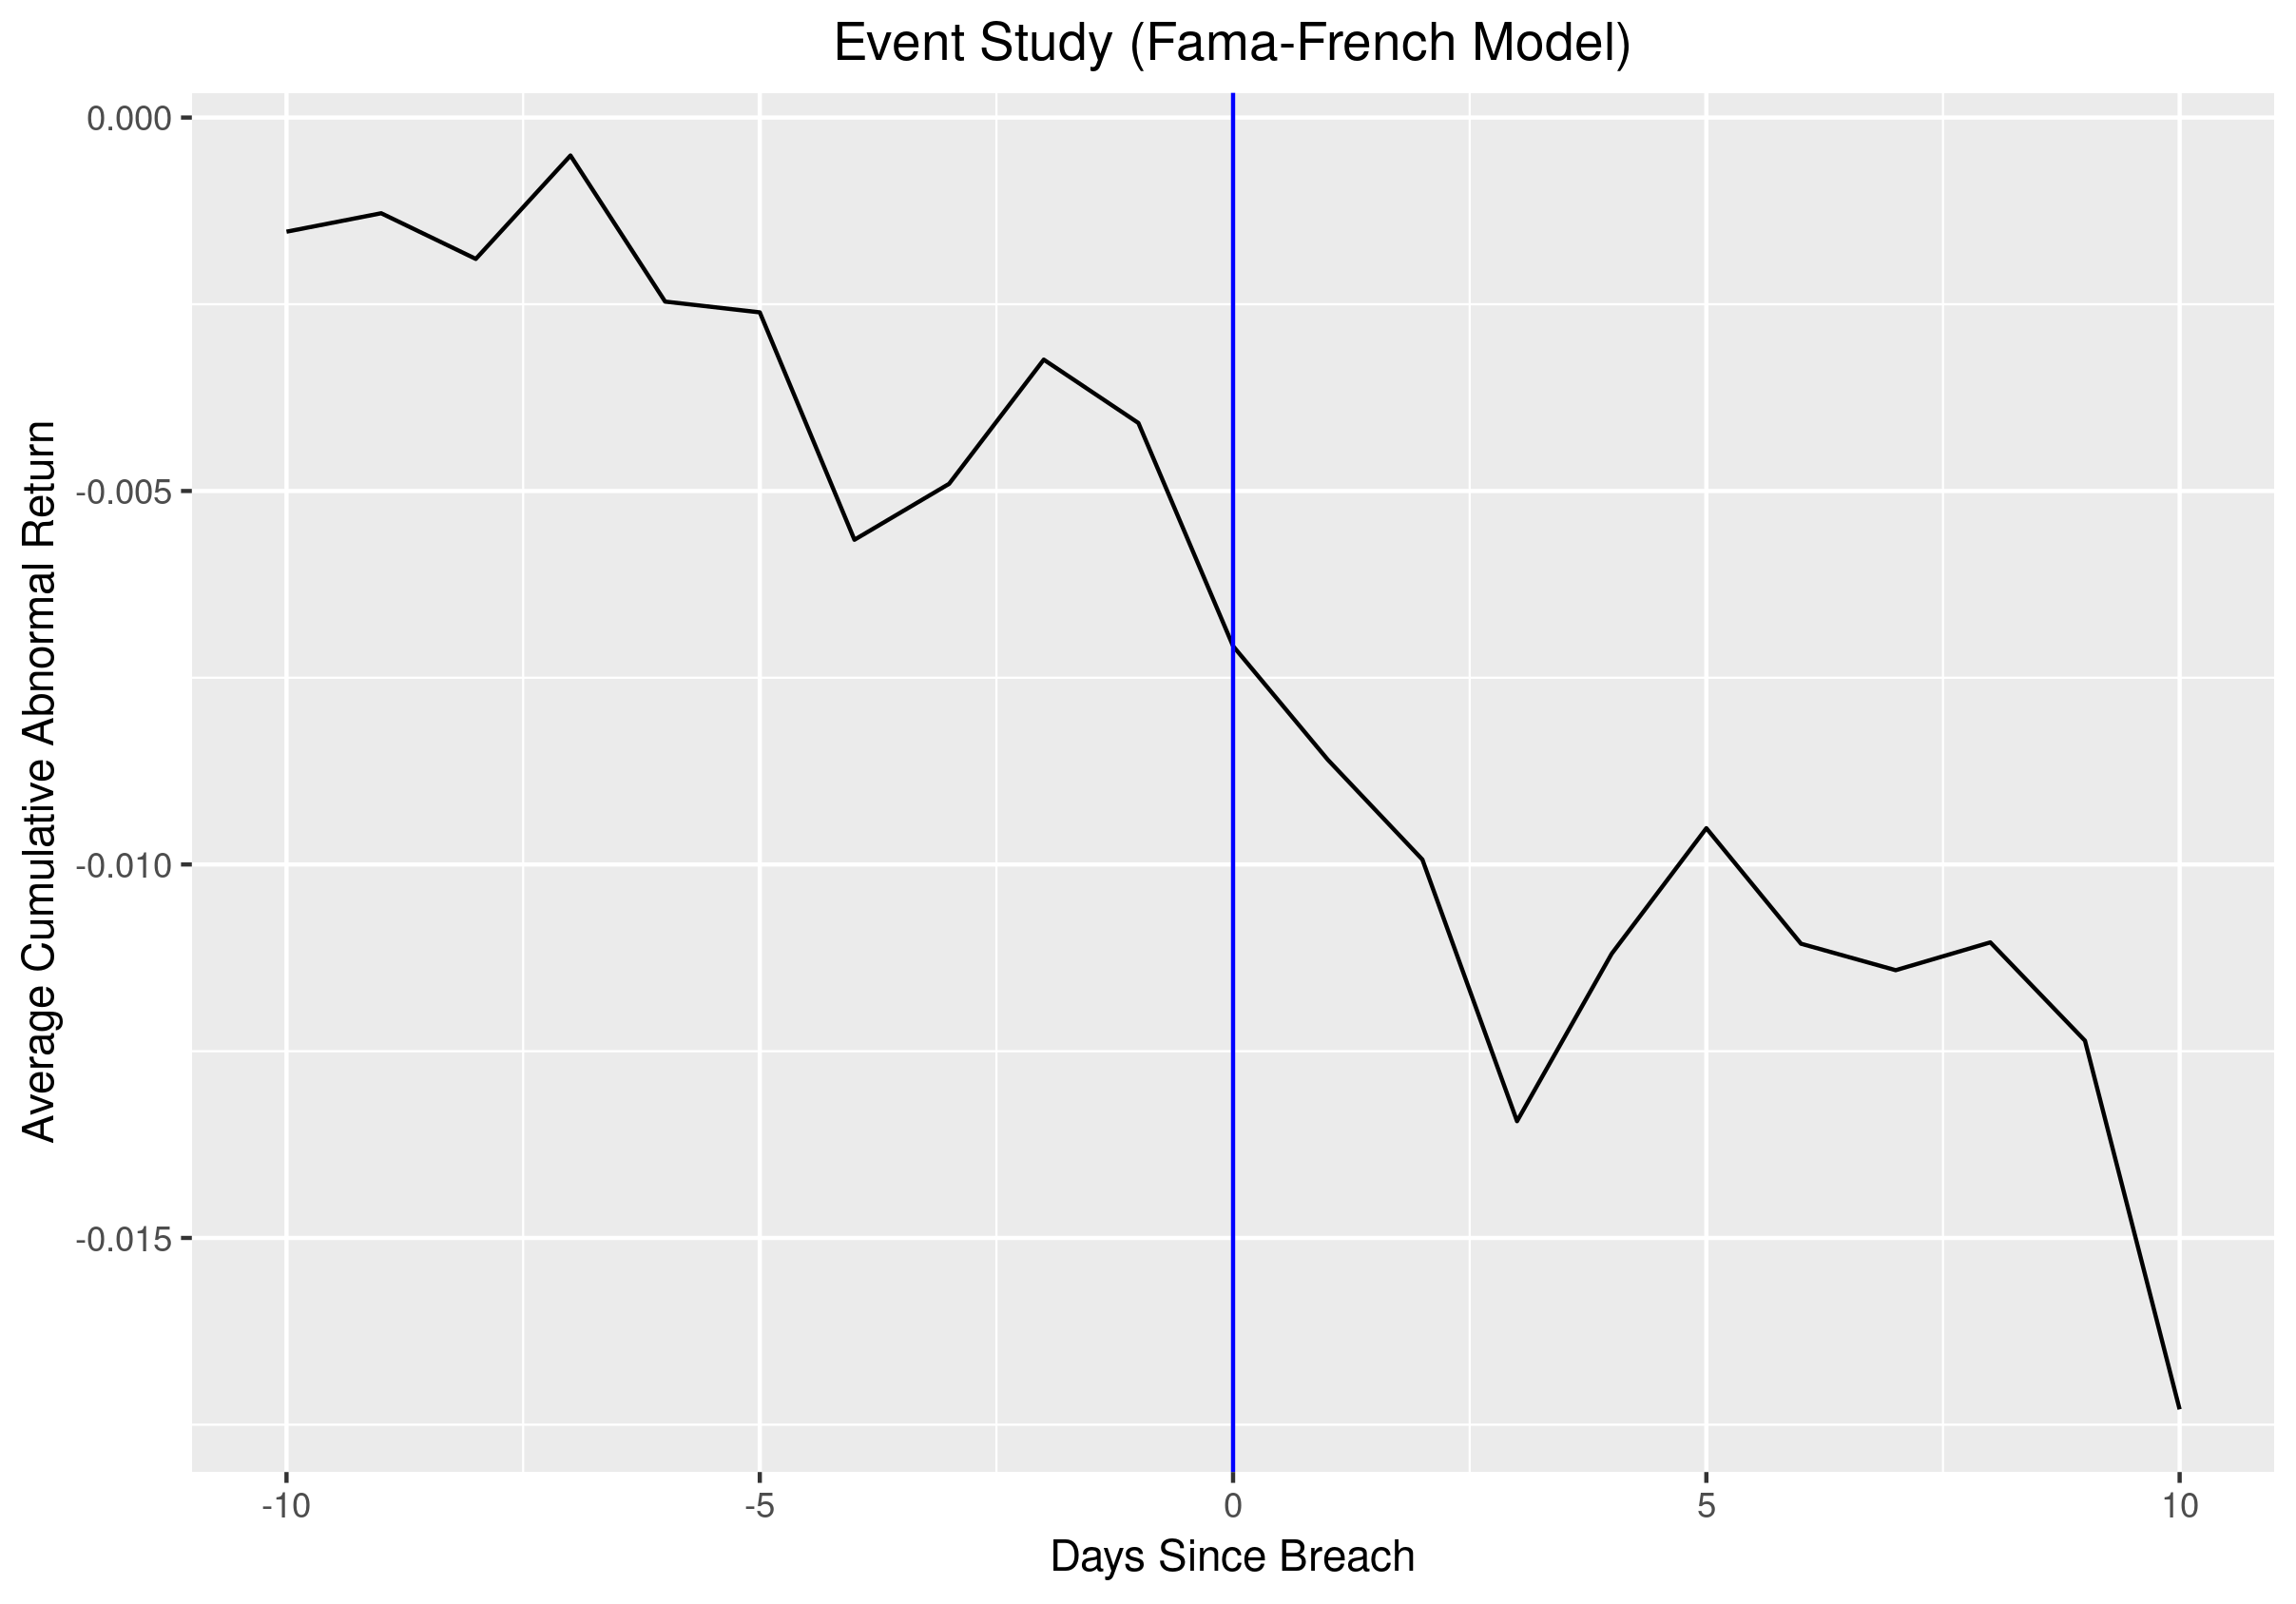
\includegraphics[width=\textwidth]{Images/ffmodel_eventstudy.png}
\end{figure}

\FloatBarrier

\begin{table}[!htbp] \centering 
  \caption{CAR t-test (CAPM Model)} 
  \label{carttestcapm} 
\resizebox{\textwidth}{!}{\begin{tabular}{@{\extracolsep{5pt}}lccccc} 
\\[-1.8ex]\hline 
\hline \\[-1.8ex] 
Event Window & 2 days & 5 days & 10 days & 90 days & 180 days \\
N & 473 & 473 & 469 & 439 & 409 \\
Mean & -0.44 & -0.54 & -0.45 & -2.03 & 0.05 \\
SD & 0.23 & 0.26 & 0.31 & 0.98 & 2.00 \\
t-stat & -1.95 & -2.08 & -1.49 & -2.07 & 0.02 \\
p & 0.03$^{**}$ & 0.02$^{**}$ & 0.07$^{*}$ & 0.02$^{**}$ & 0.51 \\
\\[-1.8ex]\hline
\hline \\[-1.8ex]
\textit{Note:}  & \multicolumn{5}{r}{$^{*}$p$<$0.1; $^{**}$p$<$0.05; $^{***}$p$<$0.01} \\ 
 & \multicolumn{5}{r}{Returns given as percentages} \\ 
\hline \\[-1.8ex] 
\end{tabular}} 
\end{table} 

\begin{table}[!htbp] \centering 
  \caption{CAR t-test (Fama -French Model)} 
  \label{carttestff} 
\resizebox{\textwidth}{!}{\begin{tabular}{@{\extracolsep{5pt}}lccccc} 
\\[-1.8ex]\hline 
\hline \\[-1.8ex] 
Event Window & 2 days & 5 days	& 10 days & 90 days & 180 days \\
N & 473 & 473 & 469 & 439 & 409 \\
Mean & -0.57 & -0.71 & -0.64 & -2.54 & -1.30 \\
SD & 0.22 & 0.25 & 0.30 & 0.93 & 1.97 \\
t-stat & -3.00 & -3.00 & -2.00 & -3.00 & -1.00 \\
p & 0.01$^{**}$ & 0.00$^{***}$ & 0.02$^{**}$ & 0.00$^{***}$ & 0.26 \\
\\[-1.8ex]\hline
\hline \\[-1.8ex]
\textit{Note:}  & \multicolumn{5}{r}{$^{*}$p$<$0.1; $^{**}$p$<$0.05; $^{***}$p$<$0.01} \\ 
 & \multicolumn{5}{r}{Returns given as percentages} \\ 
\hline \\[-1.8ex] 
\end{tabular}} 
\end{table} 

\begin{table}[!htbp] \centering 
  \caption{CAR t-test (CAPM) (with two days restriction)} 
  \label{carttesttwodaymm} 
\resizebox{\textwidth}{!}{\begin{tabular}{@{\extracolsep{5pt}}lccccc} 
\\[-1.8ex]\hline 
\hline \\[-1.8ex] 
Event Window & 2 days & 5 days & 10 days & 90 days & 180 days \\
N & 438 & 372 & 275 & 51 & 24 \\
Mean & -0.51 & -0.67 & -0.59 & -3.87 & 0.33 \\
SD & 0.22 & 0.28 & 0.39 & 3.25 & 6.82 \\
t-stat & -2.26 & -2.39 & -1.52 & -1.19 & 0.05 \\
p & 0.01$^{**}$ & 0.01$^{**}$ & 0.06$^{*}$ & 0.12 & 0.52 \\
\\[-1.8ex]\hline
\hline \\[-1.8ex]
\textit{Note:}  & \multicolumn{5}{r}{$^{*}$p$<$0.1; $^{**}$p$<$0.05; $^{***}$p$<$0.01} \\ 
 & \multicolumn{5}{r}{Returns given as percentages} \\ 
\hline \\[-1.8ex] 
\end{tabular}} 
\end{table} 

\begin{table}[!htbp] \centering 
  \caption{CAR t-test (Fama-French) (with two days restriction)} 
  \label{carttesttwodayff} 
\resizebox{\textwidth}{!}{\begin{tabular}{@{\extracolsep{5pt}}lccccc} 
\\[-1.8ex]\hline 
\hline \\[-1.8ex]
Event Window & 2 days & 5 days & 10 days & 90 days & 180 days \\
N & 438 & 372 & 275 & 51 & 24 \\
Mean & -0.65 & -0.88 & -0.84 & -3.71 & -1.38 \\
SD & 0.22 & 0.27 & 0.37 & 3.23 & 6.11 \\
t-stat & -3.00 & -3.00 & -2.00 & -1.00 & 0.00 \\
p & 0.00$^{*** }$ & 0.00$^{***}$ & 0.01$^{**}$ & 0.13 & 0.41 \\
\\[-1.8ex]\hline
\hline \\[-1.8ex]
\textit{Note:}  & \multicolumn{5}{r}{$^{*}$p$<$0.1; $^{**}$p$<$0.05; $^{***}$p$<$0.01} \\ 
 & \multicolumn{5}{r}{Returns given as percentages} \\ 
\hline \\[-1.8ex] 
\end{tabular}} 
\end{table} 

\FloatBarrier

% Table created by stargazer v.5.2.2 by Marek Hlavac, Harvard University. E-mail: hlavac at fas.harvard.edu
% Date and time: Tue, Mar 26, 2019 - 06:07:01 PM
\begin{table}[!htbp] \centering 
  \caption{Regress CAR on various explanatory factors} 
  \label{smregression} 
\resizebox{\textwidth}{!}{\begin{tabular}{@{\extracolsep{5pt}}lcccccc} 
\\[-1.8ex]\hline 
\hline \\[-1.8ex] 
 & \multicolumn{6}{c}{\textit{Dependent variable:}} \\ 
\cline{2-7} 
\\[-1.8ex] & \multicolumn{3}{c}{Mkt Model CAR} & \multicolumn{3}{c}{FF Model CAR} \\ 
\\[-1.8ex] & (1) & (2) & (3) & (4) & (5) & (6)\\ 
\hline \\[-1.8ex] 
 Days Between Jan 1, 2005 and Breach & $-$0.001 &  &  & $-$0.002 &  &  \\ 
  & (0.002) &  &  & (0.002) &  &  \\ 
  & & & & & & \\ 
 Records Leaked (log) &  & $-$0.017 &  &  & $-$0.016 &  \\ 
  &  & (0.030) &  &  & (0.030) &  \\ 
  & & & & & & \\ 
 Customer Data Leaked &  &  & $-$0.907 &  &  & $-$0.828 \\ 
  &  &  & (0.729) &  &  & (0.716) \\ 
  & & & & & & \\ 
 Employee Data Leaked &  &  & $-$0.926 &  &  & $-$0.718 \\ 
  &  &  & (0.795) &  &  & (0.781) \\ 
  & & & & & & \\ 
 Credit Card Leaked &  &  & $-$1.482$^{**}$ &  &  & $-$1.159 \\ 
  &  &  & (0.718) &  &  & (0.705) \\ 
  & & & & & & \\ 
 SSN Leaked &  &  & 0.963 &  &  & 0.853 \\ 
  &  &  & (0.666) &  &  & (0.654) \\ 
  & & & & & & \\ 
 Name Leaked &  &  & $-$0.835 &  &  & $-$0.629 \\ 
  &  &  & (0.681) &  &  & (0.669) \\ 
  & & & & & & \\ 
 Address Leaked &  &  & $-$0.447 &  &  & $-$0.536 \\ 
  &  &  & (0.645) &  &  & (0.634) \\ 
  & & & & & & \\ 
\hline \\[-1.8ex] 
Observations & 372 & 372 & 372 & 372 & 372 & 372 \\ 
R$^{2}$ & 0.050 & 0.049 & 0.078 & 0.074 & 0.072 & 0.094 \\ 
Adjusted R$^{2}$ & 0.015 & 0.015 & 0.031 & 0.041 & 0.038 & 0.047 \\ 
\hline 
\hline \\[-1.8ex] 
\textit{Note:}  & \multicolumn{6}{r}{$^{*}$p$<$0.1; $^{**}$p$<$0.05; $^{***}$p$<$0.01} \\ 
 & \multicolumn{6}{r}{Year fixed effects in all specifications} \\ 
 & \multicolumn{6}{r}{CAR from 5 day event period} \\ 
\end{tabular}} 
\end{table} 

\FloatBarrier

\biblio % Needed for referencing to working when compiling individual subfiles - Do not remove

\end{document}